\chapter{روش پیشنهادی}
\label{chap:method}

\section{مدل سیستم}
\label{sec:system-model}

سامانه چند خوشه نزدیک دارد و هر سرور لبه عضو یک خوشه است. یکی از سرورهای هر خوشه، مدیر آن است و داده سرورهای همان خوشه را دریافت می‌کند. مدیرها گزارش خوشه خود را به ریشه می‌فرستند و تصمیم بین‌خوشه‌ای را از آن دریافت می‌کنند.

کاربر می‌تواند مستقیما به لبه هر خوشه درخواست بدهد. لبه دریافت‌کننده، مبدأ ارسال است و با جدول وزن خود یک نمونه سرویس را انتخاب می‌کند. درخواست کاربر برای ورود به خوشه از ریشه یا خوشه دیگری عبور نمی‌کند.

یک سرور می‌تواند فرستنده درخواست، میزبان سرویس یا هر دو باشد. تقاضا به مبدأ و ظرفیت پردازش به نمونه مقصد مربوط است. مدیر خوشه نیز می‌تواند روی یکی از همین سرورها اجرا شود؛ منابع لازم برای کنترل، پیش از تخصیص پردازنده به کانتینرها کنار گذاشته می‌شوند.

\begin{figure}[H]
\centering
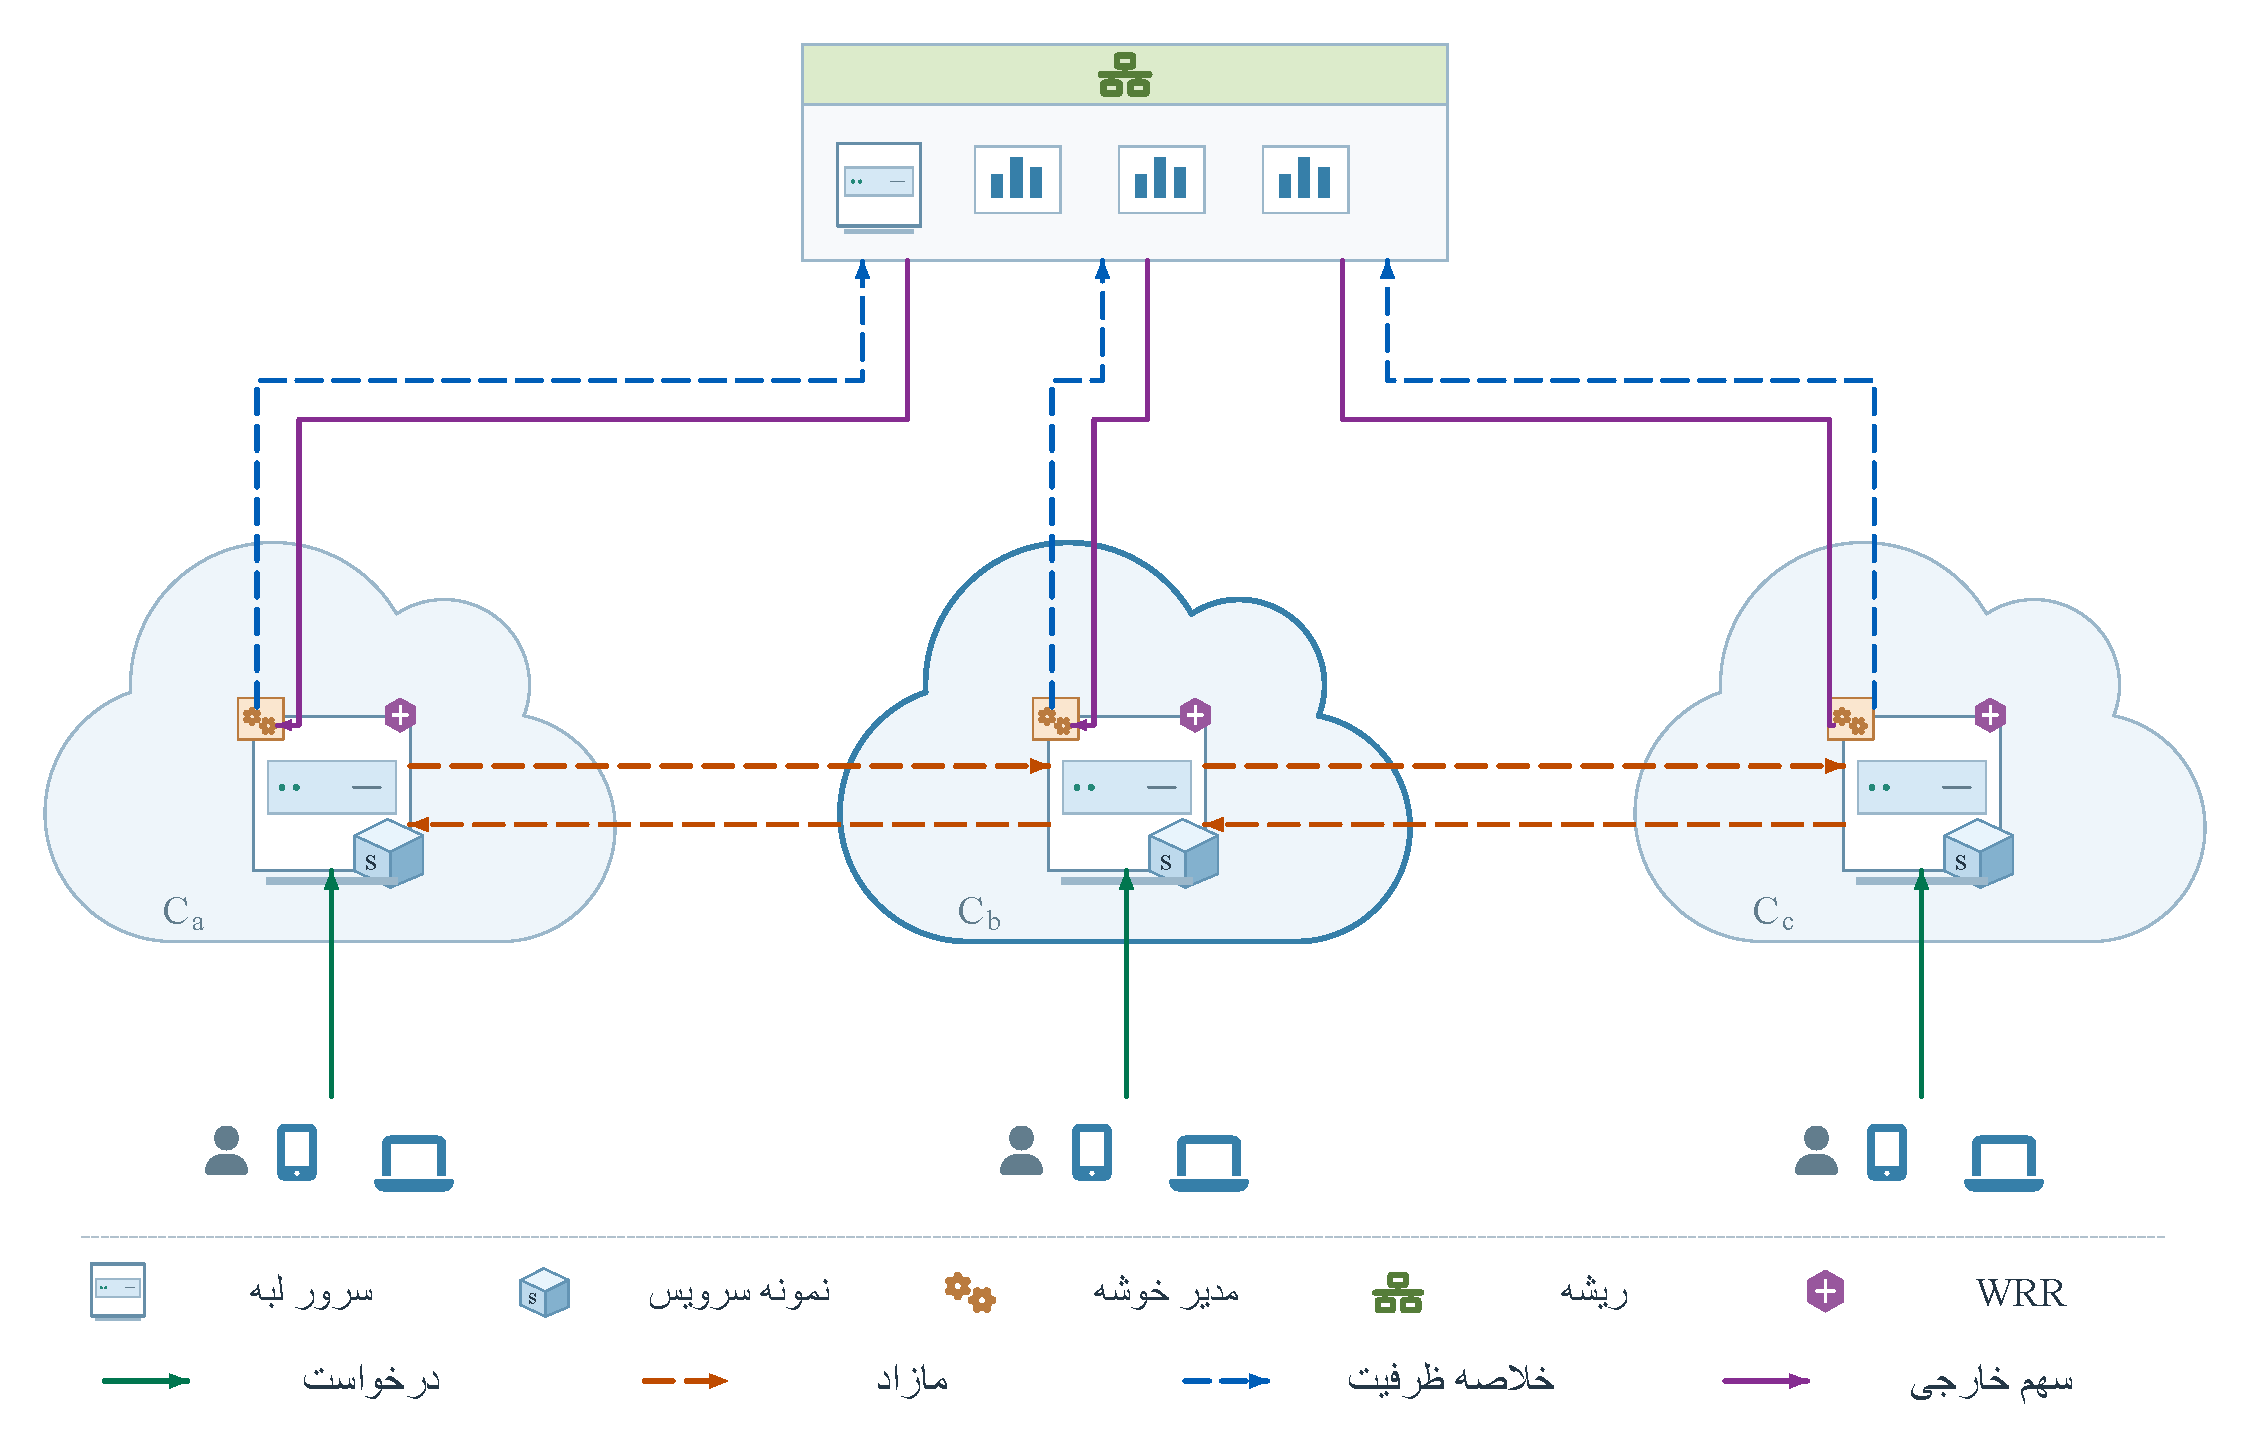
\includegraphics[width=\linewidth]{figures/visio/v10/01-system-model.pdf}
\caption[مدل سیستم و ارتباطات بین خوشه‌ها]{نمای کلی ارتباطات ریشه، خوشه‌ها و کاربران. در هر ابر یک سرور نماینده نشان داده شده است. گزارش ظرفیت به ریشه می‌رود و سهم خارجی به مدیر خوشه برمی‌گردد. پیکان‌های نارنجی بین لبه‌ها، دو زوج مسیر مستقیم ارسال مازاد را نشان می‌دهند. خوشه $C_b$ در شکل~\ref{fig:algorithm-architecture} بزرگ می‌شود.}
\label{fig:system-model}
\end{figure}

در شکل~\ref{fig:system-model}، مسیرهای خارجی برای دو زوج خوشه رسم شده‌اند؛ همین نوع ارتباط مستقیم میان هر زوج مقصد مجاز برقرار می‌شود. خوشه میانی گذرگاه درخواست خوشه‌های دیگر نیست. پیکان‌های گزارش و سهم خارجی فقط مدیرها را به ریشه وصل می‌کنند.

\subsection{اجزا، سرویس‌ها و مرز داده}

در شکل‌ها، $C_a$، $C_b$ و $C_c$ نام خوشه‌ها هستند. در روابط، $a$ و $b$ به‌ترتیب خوشه مبدأ و مقصد، $e$ مبدأ، $s$ سرویس و $i$ نمونه مقصد را نشان می‌دهند. تابع $h(i)$ میزبان فیزیکی نمونه است. هر نمونه در یک کانتینر با سهم مشخص پردازنده اجرا می‌شود و چند کانتینر می‌توانند روی یک میزبان باشند.

در روابط محلی، خوشه از متن معلوم است و شاخص آن برای کوتاه ماندن نمادهایی مانند $\mu_{si}$ تکرار نمی‌شود. در جدول بین‌خوشه‌ای، زوج $(b,i)$ نمونه مقصد را مشخص می‌کند.

اگر نمونه‌های فراخواننده روی یک لبه به سیاست جدا نیاز داشته باشند، شناسه مبدأ $e$ زوج «لبه، نمونه فراخواننده» است؛ روابط بدون افزودن شاخص تازه به کار می‌روند.

مجموعه $\mathcal E_a$ مبدأهای خوشه $a$ است. مجموعه $\mathcal A_{as}$ نمونه‌های سالم، آماده و مجاز سرویس $s$ با برآورد ظرفیت معتبر را نشان می‌دهد. میزبان‌های متمایز همین نمونه‌ها مجموعه $\mathcal H_{as}=\{h(i):i\in\mathcal A_{as}\}$ را می‌سازند؛ فرض می‌شود مبدأهای خوشه به این مجموعه مقصد مشترک دسترسی دارند.

داده خام پردازنده و صف هر سرور فقط در اختیار مدیر همان خوشه است. ریشه شناسه نمونه‌های سرویس و خلاصه ظرفیت آن‌ها را دارد. داده منابع مستقیما بین دو مدیر خوشه ردوبدل نمی‌شود.

مقصدهای خارجی باید از نظر شبکه و مجوز سرویس قابل دسترسی باشند. فهرست نمونه‌های سالم و آماده، ورودی محاسبه وزن است.

\subsection{تقاضا، ظرفیت و بار مشاهده‌شده}

پنجره پایش $\Delta$ قابل تنظیم است و در این متن مقدار پایه آن $5$ ثانیه است. هر تلاش ارسال، مستقل از موفقیت آن، یک بار در مبدأ شمرده می‌شود. اگر بازتلاش فعال باشد، شمار تلاش با شمار درخواست اصلی برنامه جدا نگه داشته می‌شود.

با $A^{\mathrm{src}}_{es}$ آغاز تلاش، نرخ مبدأ و نرخ کل تقاضای همان سرویس در خوشه عبارت‌اند از
\begin{equation}
 D_{es}=\frac{A^{\mathrm{src}}_{es}}{\Delta},\qquad
 D_{as}=\sum_{e\in\mathcal E_a}D_{es}.
 \label{eq:source-demand}
\end{equation}
واحد نرخ، درخواست بر ثانیه است. $D_{as}$ تقاضایی است که توزیع آن از لبه‌های خوشه $a$ آغاز می‌شود؛ درخواست مستقیم کاربران و فراخوانی‌های تولیدشده در این لبه‌ها را در بر می‌گیرد. شمار ورود به کانتینر مقصد، بار دریافتی آن را نشان می‌دهد؛ شمار پردازش‌های پایان‌یافته برای برآورد توان خدمت به کار می‌رود.

ورود درخواست محلی یا خارجی در کانتینر مقصد ثبت می‌شود، اما برای همان درخواست، تقاضای مبدأ دوباره ساخته نمی‌شود. نمونه مقصد درخواست را اجرا می‌کند؛ اگر سرویس دیگری را فراخوانی کند، آن فراخوانی تقاضای تازه همان سرویس است.

هر کانتینر نمونه $i$ از سرویس $s$، سهم قابل اتکای $g_{si}>0$ هسته پردازنده دارد. این سهم می‌تواند کسری از یک هسته باشد. تخصیص‌دهنده منابع باید مجموع سهم کانتینرهای هر میزبان را در هسته‌های قابل استفاده آن جا دهد؛ همین تخصیص، ورودی مدل است.

عامل پایش، مصرف پردازنده کانتینر را در پنجره قبل با $T^{\mathrm{CPU}}_{si}$، بر حسب هسته‌ثانیه، و تعداد پردازش‌های پایان‌یافته را با $N^{\mathrm{proc}}_{si}$ ثبت می‌کند. ظرفیت $\mu_{si}$ از این داده‌ها و سهم هسته، با مدل خطی بخش مدیر خوشه برآورد می‌شود.

ظرفیت هر کانتینر جدا برآورد می‌شود و بار زمینه سرویس‌های دیگر وارد مدل نمی‌شود. اعتبار این ساده‌سازی به تحقق سهم پردازنده و مناسب بودن تقریب خطی وابسته است.

\subsection{مشاهده مسیر، خطا و صف}

مدت هر تلاش با ساعت یکنواخت مبدأ از ارسال تا پاسخ، خطا یا پایان مهلت اندازه‌گیری می‌شود. پینگ، دوره مستقل و قابل تنظیم دارد. پاسخ \lr{API} به زمان پردازش داخلی نیاز ندارد و تفاضل زمان درخواست و پینگ نیز زمان دقیق صف را به دست نمی‌دهد.

برای $n_{ei}>0$ کاوش معتبر، میانگین مسیر چنین است:
\begin{equation}
 \overline d^{\mathrm{net}}_{ei}=\frac{1}{n_{ei}}\sum_{g=1}^{n_{ei}}d_{ei,g}.
 \label{eq:ping-mean}
\end{equation}
نوع کاوش و زمان آخرین مشاهده همراه مقدار نگهداری می‌شوند. نبود کاوش معتبر، پینگ صفر نیست.

اگر $C_{esi}$ پایان موفق و $F_{esi}$ پایان ناموفق باشند، نسبت شکست از همان جمعیت پایان‌ها ساخته می‌شود:
\begin{equation}
 \widehat f_{esi}=\frac{F_{esi}}{C_{esi}+F_{esi}},\qquad C_{esi}+F_{esi}>0.
 \label{eq:failure-observation}
\end{equation}
با $A_k$ آغاز و $O(t_k)$ تلاش در جریان، حسابداری پنجره برابر $O(t_{k+1})=O(t_k)+A_k-C_k-F_k$ است. در مخرج صفر، مشاهده شکست تازه ساخته نمی‌شود؛ مقدار معتبر قبلی و سن آن مشخص می‌مانند. 

در شروع، مقدار اولیه سیاست برای شکست با پرچم «بدون مشاهده» نگه داشته می‌شود. پینگ اولیه مسیر محلی نیز پیش از استفاده در هزینه، با کاوش معتبر به دست می‌آید.

عامل پایش، تعداد منتظران هر کانتینر را از درخواست‌های در حال خدمت جدا ثبت می‌کند. در صورت وجود ابزار، اختلاف زمان ورود به صف و شروع خدمت، انتظار را می‌دهد. زمان \lr{CPU} کل و سهم قابل انتساب سرویس نیز از اختلاف شمارنده‌های پنجره به دست می‌آیند.

مصرف پردازنده نسبت به سهم همان کانتینر نرمال می‌شود: $u_{si}=T^{\mathrm{CPU}}_{si}/(g_{si}\Delta)$. بنابراین، مصرف نیم هسته در کانتینری با سهم یک هسته، $u_{si}=0.5$ است؛ همین مصرف برای سهم دو هسته، $u_{si}=0.25$ است. درصد مصرف کل میزبان جای این نسبت را نمی‌گیرد.

\Needspace{12\baselineskip}
\begin{longtable}{>{\centering\arraybackslash}p{3.3cm}p{9.8cm}}
\caption{نمادهای پایه مدل سیستم}
\label{tab:system-symbols}\\
\toprule نماد & معنی \\ \midrule
$a,b$ & خوشه مبدأ و مقصد \\
$e,s,i,h(i)$ & مبدأ، سرویس، نمونه مقصد و میزبان فیزیکی آن \\
$\mathcal E_a$ & مبدأهای داخل خوشه \\
$\mathcal H_{as},\mathcal A_{as}$ & میزبان‌های متمایز و نمونه‌های مجاز سرویس در خوشه \\
$D_{es},D_{as}$ & تقاضای مبدأ و مجموع تقاضای محلی خوشه برای سرویس \\
$g_{si},T^{\mathrm{CPU}}_{si}$ & سهم هسته کانتینر و زمان مصرف آن در پنجره قبل \\
$N^{\mathrm{proc}}_{si},\mu_{si}$ & شمار پردازش‌های پایان‌یافته و ظرفیت خطی همان کانتینر \\
$\Delta$ & طول پنجره شمارش، ثانیه \\
$\overline d^{\mathrm{net}}_{ei},\widehat f_{esi}$ & میانگین پینگ مسیر و نسبت شکست مشاهده‌شده \\
\bottomrule
\end{longtable}

گزارش هر پنجره، زمان آغاز و پایان، شناسه تولیدکننده، نسخه استقرار و اعتبار مشاهده را دارد. شمارنده تجمعی به اختلاف همان پنجره تبدیل می‌شود و بازنشانی آن تشخیص داده می‌شود. داده خام تک‌درخواست برای ریشه ارسال نمی‌شود.


\section{الگوریتم پیشنهادی}
\label{sec:proposed-algorithm}

مدیر خوشه ابتدا ظرفیت نمونه‌های سرویس و وزن‌های محلی را محاسبه می‌کند. ریشه از ظرفیت آزاد خوشه‌ها، سهم مقصدهای خارجی را می‌سازد. اگر تقاضا از سقف داخلی بیشتر باشد، مدیر مبدأ فقط برای بخش مازاد از سهم ریشه استفاده می‌کند و جدول نهایی را به لبه می‌رساند.

\begin{figure}[H]
\centering
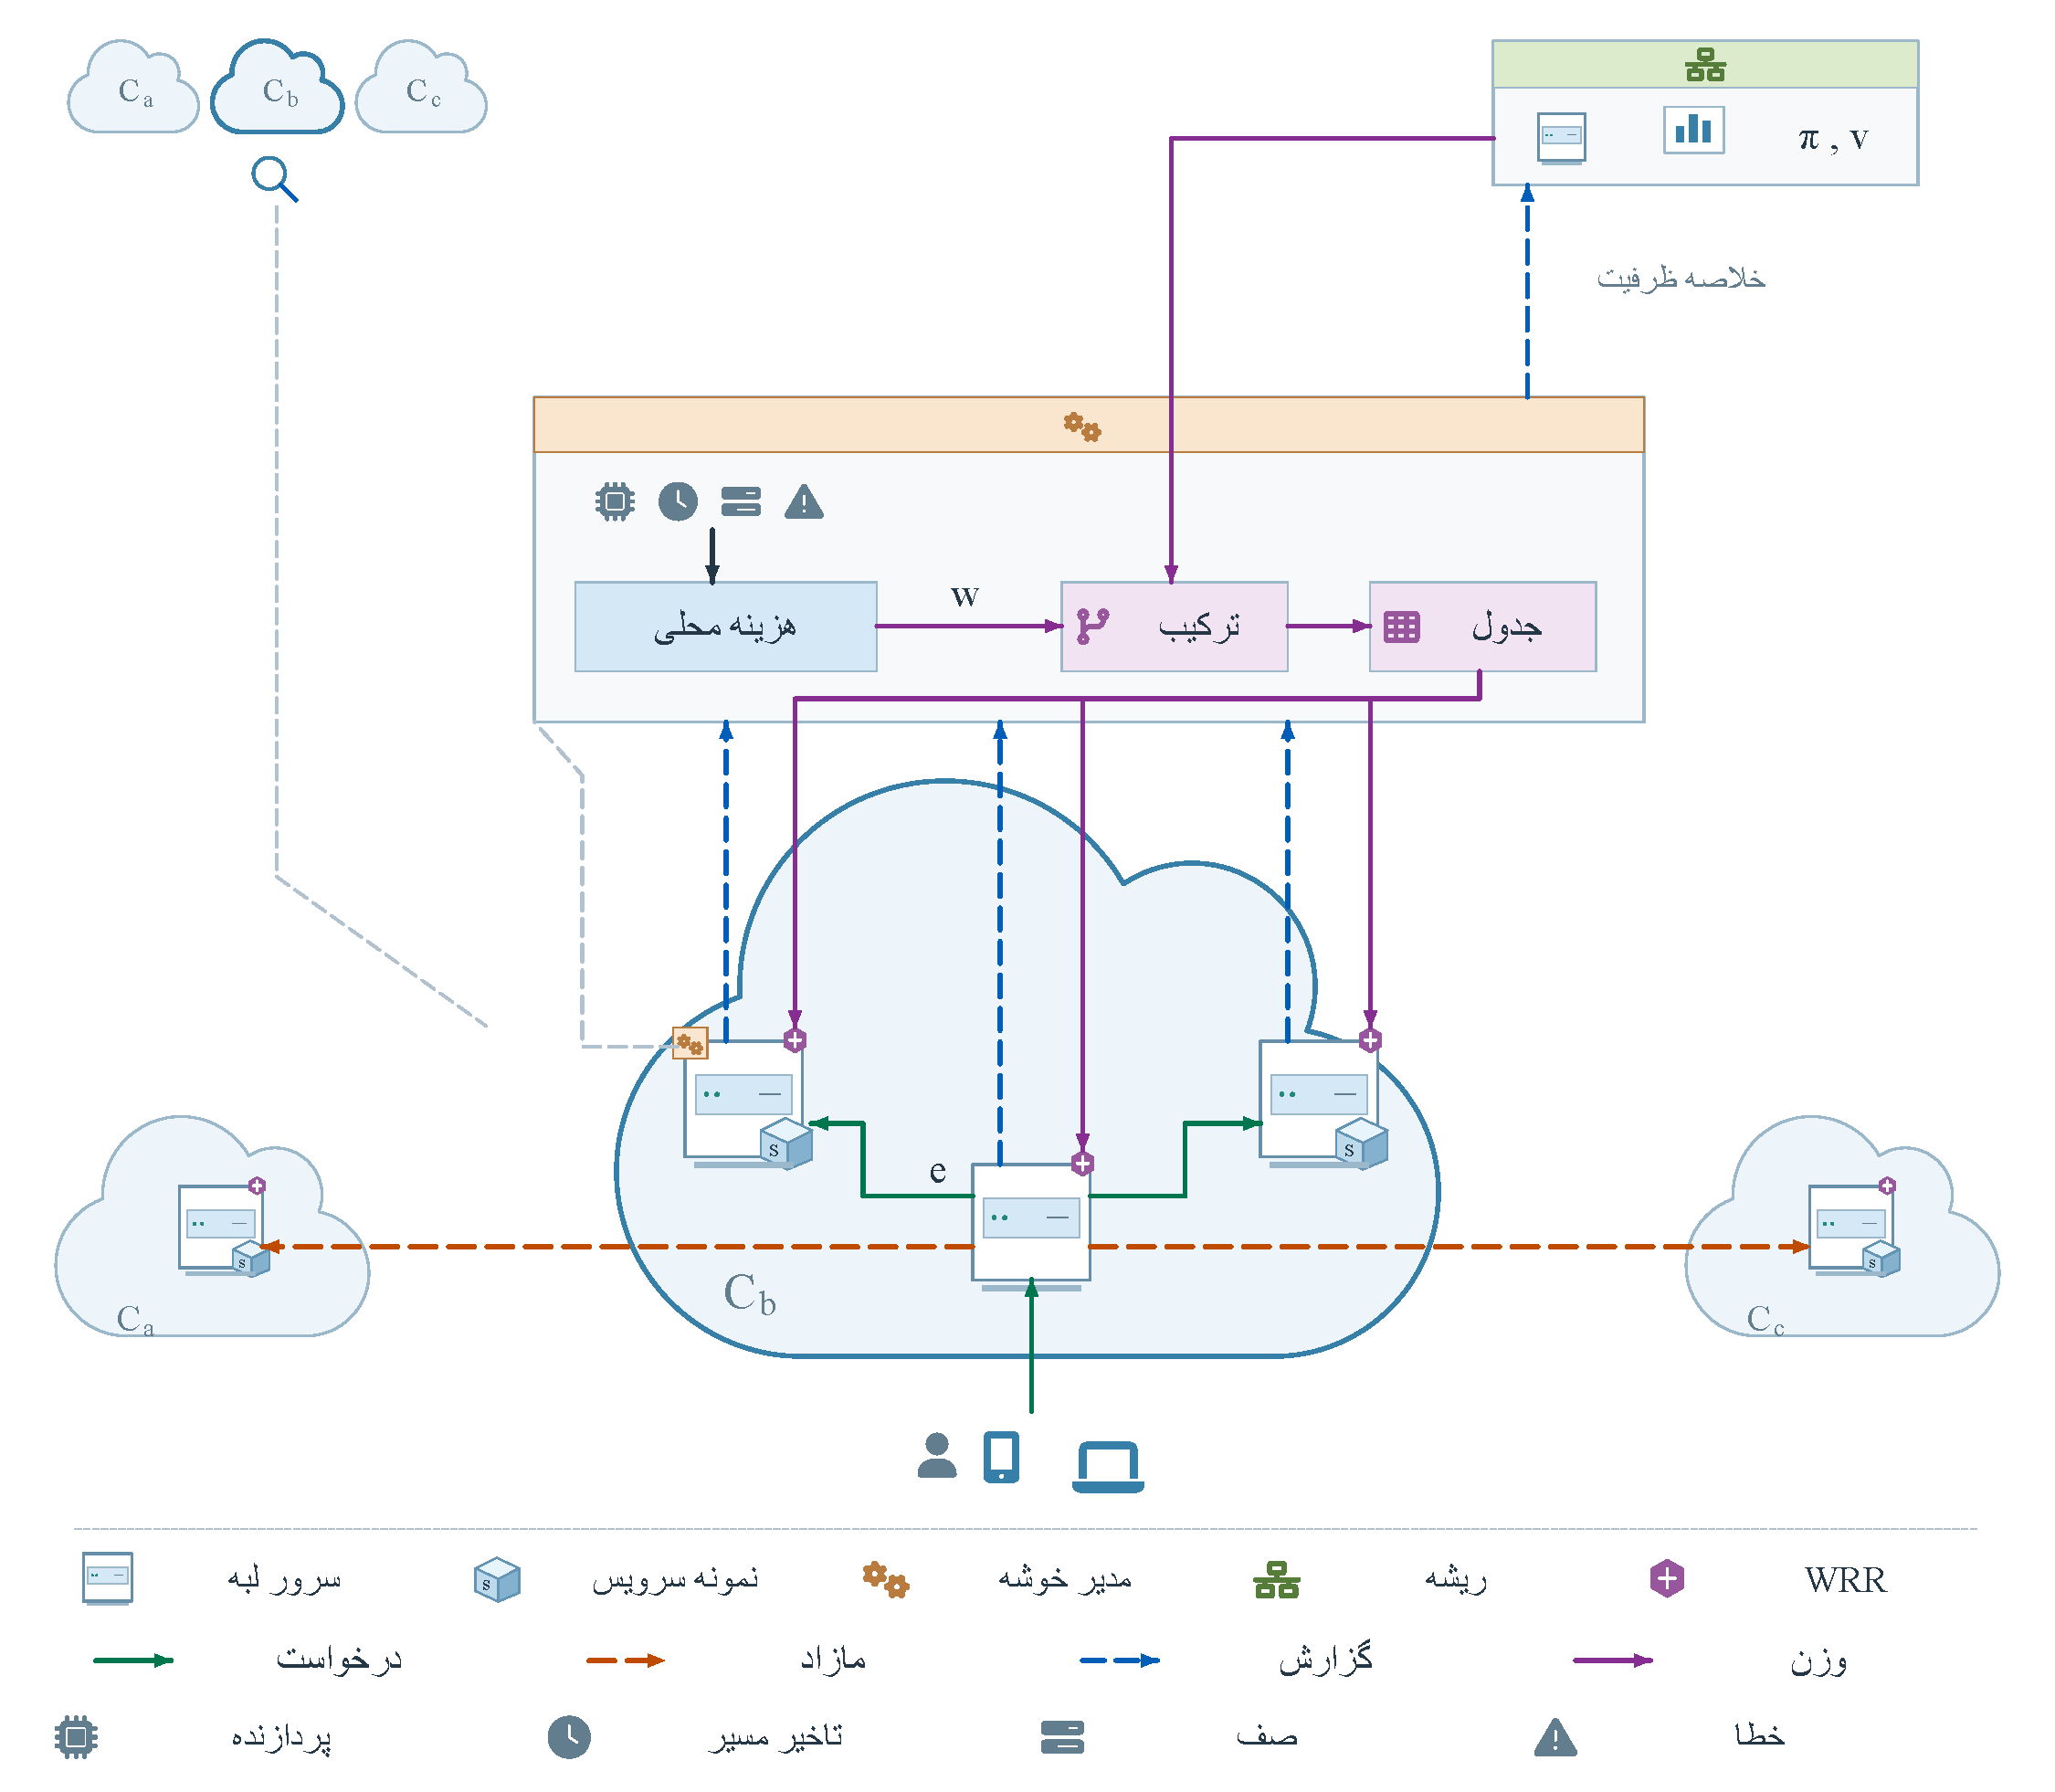
\includegraphics[width=\linewidth]{figures/visio/v10/02-algorithm-architecture.pdf}
\caption[نمای داخلی خوشه و محاسبه وزن‌ها]{نمای بزرگ‌شده خوشه $C_b$ از شکل~\ref{fig:system-model}. چرخ‌دنده روی لبه چپ، محل اجرای مدیر را نشان می‌دهد؛ کادر بالای ابر، نمای بزرگ‌شده همان مدیر است. گزارش لبه‌ها به مدیر می‌رسد؛ وزن محلی و سهم ریشه در بخش ترکیب به جدول نهایی تبدیل می‌شوند. جدول هر مبدأ به ارسال‌گر همان لبه می‌رسد. مسیرهای سبز، ارسال مستقیم محلی و مسیرهای نارنجی، ارسال مازاد به بیرون خوشه را نشان می‌دهند.}
\label{fig:algorithm-architecture}
\end{figure}

خط منشعب بنفش، انتشار جدول مخصوص هر مبدأ را نشان می‌دهد؛ وزن‌های لبه‌های مختلف لزوما یکسان نیستند. لبه با آخرین جدول معتبر و نوبت‌گردشی وزن‌دار درخواست را می‌فرستد.

\subsection{محاسبه وزن‌های محلی در مدیر خوشه}
\label{sec:cluster-manager}

مدیر خوشه برای هر مبدأ $e$ و سرویس $s$، وزن نمونه‌های داخلی را جدا محاسبه می‌کند. بنابراین، دو مبدأ می‌توانند درخواست‌های یک سرویس را با نسبت‌های متفاوت بین مقصدها تقسیم کنند. محل این محاسبه، بخش «هزینه محلی» در شکل~\ref{fig:algorithm-architecture} است.

در این بخش، $\ell_{es}$ تعداد درخواست بر ثانیه‌ای است که باید داخل خوشه پاسخ بگیرد؛ قاعده تعیین آن در بخش~\ref{sec:integration} می‌آید. ظرفیت هر مقصد به کانتینر همان سرویس تعلق دارد و در طول هر حل ثابت است.

\subsubsection{برآورد خطی ظرفیت از مصرف پردازنده}

برای هر کانتینر، سهم پردازنده $g_{si}$، زمان مصرف آن $T^{\mathrm{CPU}}_{si}$ و شمار پردازش‌های پایان‌یافته $N^{\mathrm{proc}}_{si}$ از آخرین پنجره معتبر دریافت می‌شوند. طول پیش‌فرض پنجره $\Delta=5$ ثانیه است. زمان مصرف، اختلاف شمارنده تجمعی پردازنده در آغاز و پایان همان پنجره است.

میانگین هسته مصرف‌شده، نسبت استفاده از سهم اختصاص‌یافته و نرخ پردازش مشاهده‌شده برابرند با
\begin{align}
 \overline c_{si}&=\frac{T^{\mathrm{CPU}}_{si}}{\Delta},\qquad
 u_{si}=\frac{\overline c_{si}}{g_{si}},
 \label{eq:container-utilization}\\
 y_{si}&=\frac{N^{\mathrm{proc}}_{si}}{\Delta}.
 \label{eq:processed-throughput}
\end{align}
با فرض تناسب خطی نرخ پردازش با هسته مصرف‌شده، ضریب خطی و ظرفیت کانتینر چنین به دست می‌آیند:
\begin{equation}
 \gamma_{si}=\frac{y_{si}}{\overline c_{si}}
            =\frac{N^{\mathrm{proc}}_{si}}{T^{\mathrm{CPU}}_{si}},\qquad
 \mu_{si}=\gamma_{si}g_{si}=\frac{y_{si}}{u_{si}}.
 \label{eq:cpu-linear-capacity}
\end{equation}
ضریب $\gamma_{si}$ تعداد درخواست بر ثانیه به ازای یک هسته مصرف‌شده را بیان می‌کند. مقدار $\mu_{si}$ نرخ برآوردشده در استفاده کامل از سهم پردازنده کانتینر است. اگر مصرف به صورت درصد $p_{si}$ گزارش شود، در این رابطه $u_{si}=p_{si}/100$ است.

این مدل برای ترکیب درخواست نسبتا ثابت و کار وابسته به پردازنده مناسب است. $\mu_{si}$ برآورد ظرفیت است، نه بیشینه تضمین‌شده؛ تغییر نوع درخواست یا سهم پردازنده می‌تواند آن را تغییر دهد.

اگر پردازش معتبر وجود نداشته باشد یا زمان مصرف صفر باشد، نسبت ساخته نمی‌شود. آخرین برآورد معتبر همان پیکربندی یا اندازه‌گیری راه‌اندازی به کار می‌رود. نمونه بدون برآورد معتبر در ظرفیت عادی خوشه شمرده نمی‌شود.

\subsubsection{شمار درخواست از همه مبدأها}

شمار پردازش پایان‌یافته در مقصد، همه فرستنده‌ها را پوشش می‌دهد:
\begin{equation}
 N^{\mathrm{proc}}_{si}=\sum_qN^{\mathrm{proc}}_{qsi},\qquad
 N^{\mathrm{in}}_{si}=\sum_qN^{\mathrm{in}}_{qsi},\qquad
 \lambda^{\mathrm{obs}}_{si}=\frac{N^{\mathrm{in}}_{si}}{\Delta}.
 \label{eq:all-source-observation}
\end{equation}
شاخص $q$ مبدأهای محلی و خارجی را شامل می‌شود. اگر شمارنده مقصد از ابتدا کل ورودی یا پردازش را ثبت کند، به دریافت تفکیک مبدأ نیاز نیست و جمع دوباره انجام نمی‌شود. هر تلاش در هر شمارنده مقصد فقط یک بار ثبت می‌شود.

در $N^{\mathrm{proc}}_{si}$، پردازش‌های موفق و ناموفق انجام‌شده شمرده می‌شوند؛ درخواستی که پیش از اجرا رد شده است، پردازش انجام‌شده محسوب نمی‌شود. شمار ورود ممکن است درخواست منتظر صف را هم داشته باشد؛ بنابراین در برآورد $\mu_{si}$ جای شمار پردازش پایان‌یافته را نمی‌گیرد.

نرخ $\lambda^{\mathrm{obs}}_{si}$ برای پایش و مرجع صف است و از ظرفیت کم نمی‌شود. ظرفیت از پردازش پنجره قبل برآورد می‌شود؛ حل وزن‌ها تخصیص تازه را می‌سازد و بار قبلی دوباره وارد تابع نمی‌شود.

\subsubsection{وزن‌ها، حاشیه اطمینان و سقف مشترک مبدأها}

مجموعه $\mathcal A_{es}=\mathcal A_{as}$، نمونه‌های مجاز، سالم و آماده سرویس در خوشه مبدأ با برآورد ظرفیت معتبر، مثبت و متناهی است. برای هر سطر $(e,s)$ با نرخ محلی مثبت داریم
\begin{align}
 \sum_{i\in\mathcal A_{es}}w_{esi}=1,\qquad w_{esi}&\geq0,
 \label{eq:row-weights}\\
 r_{esi}=\ell_{es}w_{esi},\qquad
 \sum_{i\in\mathcal A_{es}}r_{esi}&=\ell_{es}.
 \label{eq:load-weight}
\end{align}
هر مبدأ سطر وزن مخصوص خود را دارد؛ سقف ظرفیت مقصدها میان این سطرها مشترک است. اگر نرخ محلی صفر باشد، حل آن سطر انجام نمی‌شود و نرخ‌های محلی آن صفرند. مجموع وزن مبدأهای مختلف برای یک مقصد لازم نیست یک باشد.

با حاشیه اطمینان $0<\varepsilon<1$، سقف هر کانتینر و ظرفیت محلی سرویس عبارت‌اند از
\begin{align}
 U_{si}&=(1-\varepsilon)\mu_{si},
 \label{eq:global-cap}\\
 K_{as}&=\sum_{i\in\mathcal A_{as}}U_{si}.
 \label{eq:local-capacity}
\end{align}
هر کانتینر با سهم پردازنده خودش شمرده می‌شود؛ نرخ سرویس‌های دیگر وارد ظرفیت سرویس جاری نمی‌شود.

برای آنکه چند مبدأ ظرفیت یک کانتینر را چند بار مصرف نکنند، مجموع نرخ‌های تازه تخصیص‌یافته با $R^{\mathrm{plan}}_{si}$ نگهداری می‌شود. در آغاز حل هر سرویس، این مقدار برای همه مقصدها صفر است. مبدأها با ترتیب ثابت حل می‌شوند و سقف سطر جاری برابر است با
\begin{equation}
 R^{\mathrm{max}}_{esi}=\max\{0,U_{si}-R^{\mathrm{plan}}_{si}\}.
 \label{eq:remaining}
\end{equation}
این جمع فقط تخصیص تازه همان سرویس در همین چرخه است؛ $\mu_{si}$ در مخرج هزینه ثابت می‌ماند.

مجموعه $\cI_{es}$ مقصدهای با سقف مثبت را نشان می‌دهد. نمونه‌های بیرون از این مجموعه در حل عادی نرخ صفر دارند و برای سایر نمونه‌ها داریم
\begin{equation}
 0\leq r_{esi}\leq R^{\mathrm{max}}_{esi}\leq U_{si}<\mu_{si}.
 \label{eq:domain}
\end{equation}
ازاین‌رو، مخرج هزینه دست‌کم $\varepsilon\mu_{si}$ مثبت می‌ماند. شرط پذیرش محلی $\sum_e\ell_{es}\leq K_{as}$ در بخش ترکیب رعایت می‌شود. با مجموعه مقصد مشترک، ظرفیت باقی‌مانده پس از هر سطر برای نرخ‌های محلی حل‌نشده کافی است.

اگر $q\prec e$ مبدأهای حل‌شده پیش از مبدأ $e$ را نشان دهد، کنترل امکان تخصیص هر سطر چنین نوشته می‌شود:
\begin{equation}
 \sum_i R^{\mathrm{max}}_{esi}
   =K_{as}-\sum_{q\prec e}\ell_{qs}\geq\ell_{es}.
 \label{eq:row-feasibility}
\end{equation}
پس رزرو سطرهای قبلی، امکان تخصیص نرخ محلی سطرهای بعدی را از بین نمی‌برد.


\subsubsection{هزینه ثابت مسیر و مشاهده صف کانتینر}

هزینه ثابت هر مسیر از میانگین پینگ، جریمه شکست و مازاد انتظار صف ساخته می‌شود:
\begin{equation}
 d^{\mathrm{fix}}_{esi}=\overline d^{\mathrm{net}}_{ei}
                   +P_s\widehat f_{esi}+\delta^Q_{si}.
 \label{eq:fixed-cost}
\end{equation}
پارامتر $P_s\geq0$ جریمه تعیین‌شده برای هر شکست، بر حسب ثانیه است. پینگ و نتیجه درخواست در مبدأ ثبت می‌شوند. انتظار صف در کانتینر مقصد اندازه‌گیری می‌شود و به درج زمان پردازش در پاسخ سرویس نیاز ندارد.

برای $n_{si}^{\mathrm{start}}>0$ شروع خدمت در کانتینر، میانگین انتظار مشاهده‌شده چنین است:
\begin{equation}
 \overline W_{si}^Q=\frac{1}{n_{si}^{\mathrm{start}}}
 \sum_{j=1}^{n_{si}^{\mathrm{start}}}
 (t_j^{\mathrm{start}}-t_j^{\mathrm{enqueue}}).
 \label{eq:queue-measurement}
\end{equation}
مرجع ساده صف از مدل $M/M/1$ محاسبه می‌شود. برای حفظ مؤلفه صف روش پایه، فقط مازاد انتظار نسبت به این مرجع به هزینه ثابت افزوده می‌شود:
\begin{align}
 \lambda_{si}^{\mathrm{ref}}&=\min\{\lambda_{si}^{\mathrm{obs}},U_{si}\},\\
 W_{si}^{Q,\mathrm{ref}}&=
 \frac{\lambda_{si}^{\mathrm{ref}}}
      {\mu_{si}(\mu_{si}-\lambda_{si}^{\mathrm{ref}})},\\
 \delta^Q_{si}&=\max\{0,\overline W_{si}^Q-W_{si}^{Q,\mathrm{ref}}\}.
 \label{eq:queue-residual}
\end{align}
نرخ مرجع از کل ورودی کانتینر، شامل تمام مبدأها، ساخته می‌شود. این مرجع برای کانتینر چندرشته‌ای تقریب است؛ مازاد صف، اصلاح تجربی ثابت این چرخه است. اگر داده انتظار موجود نباشد، مؤلفه با پرچم «ناموجود» کنار گذاشته می‌شود؛ نبود داده به معنی صف اندازه‌گیری‌شده صفر نیست.

\Needspace{10\baselineskip}
\begin{longtable}{p{3.1cm}p{8.1cm}p{2.4cm}}
\caption{پارامترهای ظرفیت خطی کانتینر و تخصیص محلی}\label{tab:symbols}\\
\toprule نماد & معنا و روش تعیین & واحد \\
\midrule\endfirsthead
\multicolumn{3}{c}{ادامه جدول \ref{tab:symbols}}\\
\toprule نماد & معنا و روش تعیین & واحد \\
\midrule\endhead\bottomrule\endfoot
$g_{si}$ & سهم قابل اتکای پردازنده همان کانتینر. & هسته \\
$T^{\mathrm{CPU}}_{si}$ & زمان مصرف پردازنده در پنجره قبل. & هسته‌ثانیه \\
$N^{\mathrm{proc}}_{si}$ & کل پردازش‌های پایان‌یافته از همه مبدأها. & درخواست \\
$u_{si},y_{si}$ & نسبت مصرف سهم پردازنده و نرخ پردازش مشاهده‌شده. & نسبت؛ نرخ \\
$\gamma_{si}$ & ضریب خطی $N^{\mathrm{proc}}_{si}/T^{\mathrm{CPU}}_{si}$. & نرخ بر هسته \\
$\mu_{si},U_{si}$ & ظرفیت خطی $y_{si}/u_{si}$ و سقف با حاشیه اطمینان. & درخواست بر ثانیه \\
$\lambda^{\mathrm{obs}}_{si}$ & کل نرخ ورود کانتینر؛ برای پایش و مرجع صف. & درخواست بر ثانیه \\
$R^{\mathrm{plan}}_{si}$ & مجموع تخصیص تازه مبدأهای حل‌شده همین سرویس. & درخواست بر ثانیه \\
$R^{\mathrm{max}}_{esi}$ & ظرفیت عادی مصرف‌نشده برای سطر جاری. & درخواست بر ثانیه \\
$K_{as},\ell_{es}$ & مجموع سقف کانتینرهای محلی و نرخ پذیرفته‌شده مبدأ. & درخواست بر ثانیه \\
$d^{\mathrm{fix}}_{esi},P_s,\delta^Q_{si}$ & هزینه ثابت مسیر، جریمه شکست و مازاد صف. & ثانیه \\
$\kappa_s,r_{esi},w_{esi}$ & ضریب مثبت هزینه، نرخ تخصیص و وزن خروجی. & ضریب؛ نرخ؛ نسبت \\
\end{longtable}
در همه روابط، زمان بر حسب ثانیه و نرخ بر حسب درخواست بر ثانیه است.

\subsubsection{تابع هزینه و مسئله تخصیص}

این بخش فقط حالت $\ell_{es}\leq\sum_iR^{\mathrm{max}}_{esi}$ را حل می‌کند. نرخ نمونه‌های فاقد ظرفیت عادی صفر است و جمع‌های تابع هدف فقط روی $\cI_{es}$ انجام می‌شوند. تابع هزینه مسیر به صورت زیر است:
\begin{equation}
  C^{\mathrm{route}}_{esi}(r)
  =\frac{\kappa_s r}{\mu_{si}-r}
    +d^{\mathrm{fix}}_{esi}r,
  \qquad \kappa_s>0.
  \label{eq:route-cost}
\end{equation}
جمله کسری با نزدیک شدن نرخ تخصیص به ظرفیت کانتینر رشد می‌کند. جمله دوم، هزینه ثابت مسیر را متناسب با بار آن مسیر وارد می‌کند.

با واحدهای جدول و در نظر گرفتن شمار درخواست به عنوان کمیت شمارشی، این تابع شاخص هزینه بی‌واحد است و مستقیما زمان پاسخ یک درخواست نیست. زمان‌های شبکه، خطا و صف پیش از ترکیب، همگی به ثانیه تبدیل می‌شوند.

هدف مدیر خوشه برای زوج $(e,s)$، کمینه کردن مجموع وزن‌دار هزینه‌هاست:
\begin{equation}
  \min_{\mathbf w}\quad
  \mathcal C_{es}(\mathbf w)
  =\sum_{i\in\cI_{es}}
     w_{esi}C^{\mathrm{route}}_{esi}(\ell_{es}w_{esi}),
  \label{eq:weighted-objective}
\end{equation}
با قیود~\eqref{eq:row-weights} و~\eqref{eq:domain}.

برای ساده شدن حل، متغیر نرخ به جای وزن به کار می‌رود. با جایگذاری $w_{esi}=r_{esi}/\ell_{es}$ داریم
\begin{equation}
  \mathcal C_{es}
  =\frac{1}{\ell_{es}}
   \sum_{i\in\cI_{es}}\left[
     \frac{\kappa_s r_{esi}^{2}}
          {\mu_{si}-r_{esi}}
      +d^{\mathrm{fix}}_{esi}r_{esi}^{2}\right].
  \label{eq:objective-substitution}
\end{equation}
ضریب $1/\ell_{es}$ ثابت و مثبت است و حذف آن محل کمینه را تغییر نمی‌دهد. تابع زیر، سهم هر مقصد در هدف تبدیل‌شده را نشان می‌دهد:
\begin{equation}
  \Psi_{esi}(r)
  =\frac{\kappa_s r^2}{\mu_{si}-r}
    +d^{\mathrm{fix}}_{esi}r^2.
  \label{eq:allocation-cost}
\end{equation}
بنابراین، مسئله معادل به صورت زیر نوشته می‌شود:
\begin{equation}
\begin{aligned}
  \min_{\mathbf r}\quad &
       \Phi_{es}(\mathbf r)=\sum_{i\in\cI_{es}}\Psi_{esi}(r_{esi})\\
  \text{با قیود}\quad &
       \sum_{i\in\cI_{es}}r_{esi}=\ell_{es},\\
  &0\leq r_{esi}\leq R^{\mathrm{max}}_{esi}.
\end{aligned}
  \label{eq:allocation-problem}
\end{equation}
توان دوم از ضرب وزن در تابع هزینه و تغییر متغیر حاصل شده است. نرخ ورودی این حل، سهم محلی پذیرفته‌شده است؛ درخواست‌های بیرون از این سهم وارد تابع کسری نمی‌شوند.

\subsubsection{تحدب تابع هدف}

در این بخش، ظرفیت کانتینرها، سقف‌های تخصیص و هزینه‌های ثابت هر حل ثابت‌اند. برای کوتاه شدن روابط، شاخص‌ها حذف می‌شوند و $\mu$، $d$ و $\kappa$ به‌ترتیب ظرفیت کانتینر، هزینه ثابت و ضریب مثبت جمله کسری را نشان می‌دهند.

\Needspace{12\baselineskip}
\begin{proposition}
اگر $\kappa>0$، $\mu>0$ و $d\geq0$ باشند، تابع
$\Psi(r)=\kappa r^2/(\mu-r)+dr^2$
در ناحیه $0\leq r\leq R^{\mathrm{max}}<\mu$ اکیدا محدب است. مشتق دوم این تابع نیز در همین ناحیه اکیدا صعودی است.
\end{proposition}
\begin{proof}
مشتق اول، دوم و سوم تابع عبارت‌اند از
\begin{align}
  \Psi'(r)&=\frac{\kappa r(2\mu-r)}{(\mu-r)^2}+2dr,
    \label{eq:first-derivative}\\
  \Psi''(r)&=\frac{2\kappa\mu^2}{(\mu-r)^3}+2d>0,
    \label{eq:second-derivative}\\
  \Psi'''(r)&=\frac{6\kappa\mu^2}{(\mu-r)^4}>0.
    \label{eq:third-derivative}
\end{align}
در ناحیه مجاز، $\mu-r$ مثبت است. با توجه به $\kappa>0$ و $d\geq0$، رابطه~\eqref{eq:second-derivative} مثبت بودن مشتق دوم و در نتیجه تحدب اکید را نشان می‌دهد. رابطه~\eqref{eq:third-derivative} نیز صعودی بودن مشتق دوم را بیان می‌کند.

مجموع توابع $\Psi_{esi}$ اکیدا محدب است و قیود مسئله~\eqref{eq:allocation-problem} خطی‌اند. ناحیه مجاز، در صورت ناتهی بودن، بسته و کراندار است. بنابراین، حل همین سطر کمینه سراسری یکتا دارد.
\end{proof}

مثبت بودن مشتق دوم، تحدب اکید را ثابت می‌کند؛ مثبت بودن مشتق سوم، صعودی بودن مشتق دوم را نشان می‌دهد. این نتیجه به حل همان سطر با ورودی‌های ثابت مربوط است.

\subsubsection{حل با روش لاگرانژ و نوشتن دستگاه معادلات}
\label{sec:lagrange-system}

برای مبدأ $e$ و میکروسرویس $s$، تعداد نمونه‌های مجاز را $n$ می‌گیریم و در این دستگاه آن‌ها را با شماره‌های $1$ تا $n$ نشان می‌دهیم. تابع هدف وزنی و تابع هدف بر حسب نرخ، از رابطه $\mathcal C_{es}(\mathbf w)=\Phi_{es}(\ell_{es}\mathbf w)/\ell_{es}$ به هم مربوط‌اند.

ابتدا حالتی را می‌نویسیم که جواب در داخل بازه مجاز باشد. قید مجموع وزن‌ها خطی است و مشتق آن نسبت به هر وزن برابر یک است؛ پس برای این حالت می‌توان شرط لاگرانژ را نوشت. مقصدهایی که به سقف می‌رسند، در ادامه جدا بررسی می‌شوند.

\textbf{نوشتن تابع لاگرانژ.}
تابع هدف~\eqref{eq:weighted-objective} را بر حسب وزن‌ها باز می‌کنیم و قید مجموع وزن‌ها را با ضریب $\lambda_{es}\in\mathbb R$ به آن اضافه می‌کنیم:
\begin{equation}
\begin{aligned}
 \mathcal L(\mathbf w,\lambda_{es})={}&
 \sum_{i=1}^{n}\left[
 \frac{\kappa_s\ell_{es}w_{esi}^{2}}
      {\mu_{si}-\ell_{es}w_{esi}}
 +d^{\mathrm{fix}}_{esi}\ell_{es}w_{esi}^{2}\right]\\
 &+\lambda_{es}\left(\sum_{i=1}^{n}w_{esi}-1\right).
\end{aligned}
 \label{eq:lagrangian}
\end{equation}
برای دیدن ارتباط این لاگرانژ با تابع $\Phi_{es}$ در رابطه~\eqref{eq:allocation-problem}، کافی است $\mathbf w=\mathbf r/\ell_{es}$ را جایگذاری کنیم:
\begin{equation}
 \ell_{es}\mathcal L\left(\frac{\mathbf r}{\ell_{es}},\lambda_{es}\right)
 =\Phi_{es}(\mathbf r)
  +\lambda_{es}\left(\sum_{i=1}^{n}r_{esi}-\ell_{es}\right).
 \label{eq:lagrange-scaling}
\end{equation}
سمت راست، تابع هدف بر حسب نرخ و قید مجموع نرخ‌هاست. چون $\ell_{es}$ ثابت و مثبت است، دو نوشتار یک جواب می‌دهند.

\textbf{صفر قرار دادن مشتق‌ها.}
مشتق نسبت به هر وزن و سپس نسبت به $\lambda_{es}$ برابر صفر قرار می‌گیرد:
\begin{equation}
\begin{aligned}
 \frac{\partial\mathcal L}{\partial w_{esi}}
 &={\frac{\kappa_s\ell_{es}w_{esi}
           (2\mu_{si}-\ell_{es}w_{esi})}
          {(\mu_{si}-\ell_{es}w_{esi})^{2}}}
   +2d^{\mathrm{fix}}_{esi}\ell_{es}w_{esi}
   +\lambda_{es}=0,\\
 \frac{\partial\mathcal L}{\partial\lambda_{es}}
 &=\sum_{i=1}^{n}w_{esi}-1=0.
\end{aligned}
 \label{eq:weight-stationarity}
\end{equation}
معادله اول برای تک‌تک مقصدها نوشته می‌شود. این مشتق با جایگذاری $r=\ell_{es}w_{esi}$ در مشتق رابطه~\eqref{eq:first-derivative} به دست می‌آید و سپس $\lambda_{es}$ به آن اضافه می‌شود. معادله دوم نیز مجموع وزن‌ها را یک نگه می‌دارد.

\textbf{تشکیل دستگاه معادلات.}
با جایگذاری $r_{esi}=\ell_{es}w_{esi}$، جمله $\ell_{es}w_{esi}$ در مشتق‌ها به $r_{esi}$ تبدیل می‌شود. قید مجموع نیز به صورت $\sum_i r_{esi}=\ell_{es}\sum_iw_{esi}=\ell_{es}$ درمی‌آید. بنابراین، دستگاه زیر به دست می‌آید:
\begin{equation}
\left\{
\begin{aligned}
 &\frac{\kappa_s r_{es1}(2\mu_{s1}-r_{es1})}
        {(\mu_{s1}-r_{es1})^{2}}
       +2d^{\mathrm{fix}}_{es1}r_{es1}=-\lambda_{es},\\[4pt]
 &\frac{\kappa_s r_{es2}(2\mu_{s2}-r_{es2})}
        {(\mu_{s2}-r_{es2})^{2}}
       +2d^{\mathrm{fix}}_{es2}r_{es2}=-\lambda_{es},\\[2pt]
 &\hspace{4cm}\vdots\\[2pt]
 &\frac{\kappa_s r_{esn}(2\mu_{sn}-r_{esn})}
        {(\mu_{sn}-r_{esn})^{2}}
       +2d^{\mathrm{fix}}_{esn}r_{esn}=-\lambda_{es},\\[4pt]
 &r_{es1}+r_{es2}+\cdots+r_{esn}=\ell_{es}.
\end{aligned}
\right.
 \label{eq:rate-system}
\end{equation}
این دستگاه $n+1$ معادله و $n+1$ مجهول دارد: نرخ‌های $r_{es1}$ تا $r_{esn}$ و ضریب $\lambda_{es}$. ظرفیت‌ها، هزینه‌های مسیر و نرخ تقاضا در این مرحله معلوم‌اند. اگر جواب در داخل بازه مجاز باشد، با توجه به تحدب اکید، نرخ‌های به‌دست‌آمده کمینه یکتای همین مسئله‌اند.

\textbf{بررسی جواب مقید.}
دستگاه~\eqref{eq:rate-system} برای مقصدهایی نوشته شده است که نرخ آن‌ها مثبت و کمتر از سقف باشد. اگر جواب روی مرز قرار بگیرد، برابری مشتق همه مقصدها لازم نیست. برای بیان یکسان این حالت‌ها، مشتق هزینه هر مقصد را با $M_{esi}$ مشخص می‌کنیم:
\begin{equation}
 M_{esi}(r)=
 \frac{\kappa_s r(2\mu_{si}-r)}
      {(\mu_{si}-r)^{2}}
 +2d^{\mathrm{fix}}_{esi}r.
 \label{eq:marginal}
\end{equation}
با تعریف $\nu_{es}=-\lambda_{es}$، جواب معتبر برای مقصدهای دارای سقف مثبت، شرط‌های زیر را رعایت می‌کند:
\begin{equation}
\begin{aligned}
 M_{esi}(r_{esi})&\begin{cases}
 \geq\nu_{es},&r_{esi}=0,\\
 =\nu_{es},&0<r_{esi}<R^{\mathrm{max}}_{esi},\\
 \leq\nu_{es},&r_{esi}=R^{\mathrm{max}}_{esi},
 \end{cases}\\
 \sum_{i\in\cI_{es}}r_{esi}&=\ell_{es},\qquad
 0\leq r_{esi}\leq R^{\mathrm{max}}_{esi}.
\end{aligned}
 \label{eq:optimality-conditions}
\end{equation}
به دلیل تحدب اکید و خطی بودن قیود، هر جواب مجاز با این شرط‌ها، کمینه یکتای همان سطر است.

اگر تقاضا برابر مجموع سقف‌ها باشد، نرخ همه مقصدها از همان سقف‌ها مشخص می‌شود. در این حالت، ممکن است بیش از یک مقدار برای ضریب لاگرانژ معتبر باشد؛ یکتایی نرخ‌ها به معنی یکتایی این ضریب نیست.

روش حل آزاد است؛ جواب باید قیود و شرط‌های~\eqref{eq:optimality-conditions} را با دقت مشخص رعایت کند.

وزن نهایی هر مقصد از نرخ حل‌شده به دست می‌آید:
\begin{equation}
 w_{esi}^{\star}=\frac{r_{esi}^{\star}}{\ell_{es}}.
 \label{eq:final-weights}
\end{equation}
دقت حل و خطای مجاز قید مجموع باید مشخص شوند. پس از گرد کردن وزن‌ها برای اجرا نیز مجموع سطر و سقف مقصدها دوباره بررسی می‌شود؛ تغییر ساده وزن‌ها برای یک شدن مجموع، به‌تنهایی رعایت سقف‌ها را تضمین نمی‌کند.


\subsubsection{اثر پارامترها بر وزن‌ها}
\label{sec:parameter-effects}

اثرهای جدول برای یک سطر با ثابت بودن سایر داده‌ها و سقف‌ها بیان می‌شوند. ظرفیت و سقف هر کانتینر از پایش و تخصیص هسته به دست می‌آیند. با تغییر هر ورودی، وزن‌ها از حل دوباره همان مسئله تعیین می‌شوند.

\Needspace{10\baselineskip}
\begin{longtable}{p{3.2cm}p{10.8cm}}
\caption{اثر پارامترهای کانتینر و مسیر بر تخصیص}\label{tab:local-effects}\\
\toprule پارامتر & اثر تغییر \\
\midrule\endfirsthead
\multicolumn{2}{c}{ادامه جدول \ref{tab:local-effects}}\\
\toprule پارامتر & اثر تغییر \\
\midrule\endhead\bottomrule\endfoot
$\overline d^{\mathrm{net}}_{ei}$ & افزایش پینگ، وزن همان مقصد را کاهش می‌دهد یا ثابت می‌گذارد؛ کاهش پینگ جهت معکوس دارد. \\
$\widehat f_{esi},\delta^Q_{si}$ & با $P_s>0$، افزایش شکست، وزن همان مقصد را کاهش می‌دهد یا ثابت می‌گذارد. افزایش مازاد صف نیز همین اثر را دارد و به مثبت بودن $P_s$ وابسته نیست. \\
$\mu_{si}$ & با افزایش ظرفیت و ثابت بودن هزینه مسیر، فشار هزینه در نرخ ثابت کمتر می‌شود؛ با بازتر شدن سقف، وزن همان مقصد کاهش نمی‌یابد. \\
$R^{\mathrm{max}}_{esi}$ & افزایش سقف، امکان تخصیص بیشتر می‌دهد؛ اگر سقف فعال نباشد، تغییر کوچک آن بی‌اثر است. \\
$g_{si}$ & با ثابت بودن ضریب $\gamma_{si}$، افزایش سهم هسته ظرفیت را خطی بیشتر می‌کند. افزایش سهم تخصیصی باید واقعا در اختیار کانتینر قرار گیرد. \\
$N^{\mathrm{proc}}_{si}$ & با ثابت بودن زمان مصرف و سهم هسته، افزایش شمار پردازش، ظرفیت برآوردشده را بیشتر می‌کند. این اثر، مقایسه جبری ورودی‌هاست و به معنی ثابت ماندن مصرف در هر اجرای واقعی نیست. \\
$T^{\mathrm{CPU}}_{si}$ & با ثابت بودن شمار پردازش و سهم هسته، مصرف بیشتر یعنی هزینه پردازنده بیشتر برای هر درخواست و ظرفیت خطی کمتر. \\
\end{longtable}

\Needspace{10\baselineskip}
\begin{longtable}{p{3.2cm}p{10.8cm}}
\caption{اثر پارامترهای مشترک حل محلی}\label{tab:shared-effects}\\
\toprule پارامتر & نقش \\
\midrule\endfirsthead
\multicolumn{2}{c}{ادامه جدول \ref{tab:shared-effects}}\\
\toprule پارامتر & نقش \\
\midrule\endhead\bottomrule\endfoot
$\ell_{es}$ & با سقف‌های ثابت، افزایش تقاضا نرخ تخصیص مقصدها را کاهش نمی‌دهد؛ وزن نسبی آن‌ها می‌تواند کم یا زیاد شود. \\
$\varepsilon$ & افزایش حاشیه اطمینان، سقف‌ها و ظرفیت قابل پذیرش محلی را کمتر می‌کند. اثر هر وزن به سقف‌های فعال وابسته است. \\
$P_s$ & افزایش آن اهمیت خطا را بیشتر می‌کند؛ جهت تغییر تک‌تک وزن‌ها به نسبت شکست و نرخ همه مقصدها وابسته است. \\
$\kappa_s$ & افزایش این ضریب، اهمیت جمله کسری را نسبت به هزینه ثابت بیشتر می‌کند. جهت تغییر هر وزن عمومی نیست. \\
$\Delta$ & طول پنجره بر تازگی و نوسان اندازه‌گیری اثر دارد. با شمارش و زمان مصرف یک پنجره مشترک، نسبت $N^{\mathrm{proc}}/T^{\mathrm{CPU}}$ به طور مستقیم ضریب جداگانه‌ای از $\Delta$ ندارد. \\
\end{longtable}
نسبت مصرف و نرخ پردازش مستقل از هم نیستند؛ هر دو از همان پنجره ساخته می‌شوند. افزایش مصرف به‌تنهایی نشانه کاهش ظرفیت نیست؛ اگر نرخ پردازش نیز به همان نسبت زیاد شود، برآورد ظرفیت ثابت می‌ماند.

\subsubsection{ثبت تخصیص تازه و پایان محاسبه محلی}

پس از حل سطر $(e,s)$، نرخ‌های تازه در جمع تخصیص همان سرویس ثبت می‌شوند:
\begin{equation}
 R^{\mathrm{plan}}_{si}\gets R^{\mathrm{plan}}_{si}+r_{esi}^{\star}.
 \label{eq:planned-update}
\end{equation}
سطر بعدی از سقف باقی‌مانده همین کانتینر استفاده می‌کند. در پایان حل همه مبدأهای محلی، داریم
\begin{equation}
 R^{\mathrm{plan}}_{si}=\sum_{e\in\mathcal E_a}r_{esi}^{\star}\leq U_{si}.
 \label{eq:aggregate-plan}
\end{equation}
پس جمع نرخ ارسالی همه مبدأها به یک کانتینر از سقف آن بیشتر نمی‌شود. برای سرویس دیگر، جمع تخصیص از صفر آغاز می‌شود و نرخ سرویس قبلی وارد آن نمی‌شود.

ترتیب مبدأها ثابت و ثبت‌شده است. هر سطر با ورودی ثابت، کمینه یکتای خودش را دارد؛ نتیجه کل به ترتیب سطرها وابسته است و کمینه مشترک همه مبدأها ادعا نمی‌شود. جمله کسری، شاخص هزینه تخصیص همین مبدأ است و زمان دقیق صف ناشی از مجموع همه ورودی‌ها نیست.

خروجی این بخش وزن شرطی نمونه‌های محلی است. در ظرفیت کافی، همین وزن‌ها برای ارسال محلی کافی‌اند. برای بخش مازاد تقاضا، سهم خوشه‌های پذیرنده لازم است؛ بخش بعد محاسبه آن را در ریشه توضیح می‌دهد.

\subsection{محاسبه سهم خوشه‌ها و نمونه‌های خارجی در ریشه}
\label{sec:root}

ریشه در شکل~\ref{fig:algorithm-architecture} سهم مقصدهای خارجی را تعیین می‌کند. مدیر هر خوشه ابتدا بار محلی را تخصیص می‌دهد و ظرفیت باقی‌مانده نمونه‌ها را گزارش می‌کند. ریشه این ظرفیت‌های آزاد را به سهم تبدیل می‌کند؛ مدیر مبدأ فقط برای مازاد تقاضای داخلی از آن‌ها استفاده می‌کند.

\subsubsection{گزارش ظرفیت خالی هر نمونه}

پس از محاسبه تخصیص محلی، مدیر خوشه $b$ ظرفیت قابل عرضه هر نمونه $i$ از سرویس $s$ را محاسبه می‌کند:
\begin{equation}
 S_{bsi}=\max\{0,U_{si}-R^{\mathrm{plan}}_{si}\},\qquad
 A_{bs}=\sum_{i\in\mathcal A_{bs}}S_{bsi}.
 \label{eq:root-available}
\end{equation}
$U_{si}$ سقف نمونه پس از حاشیه اطمینان، $R^{\mathrm{plan}}_{si}$ بار محلی تخصیص‌یافته و $S_{bsi}$ ظرفیت آزاد قابل عرضه است. $A_{bs}$ جمع این ظرفیت آزاد در خوشه است. واحد همه آن‌ها درخواست بر ثانیه است؛ حاشیه اطمینان دوباره کم نمی‌شود.

مدیر خوشه، $S_{bsi}$ را همراه شناسه سرویس، نمونه و میزبان به ریشه می‌فرستد. این ظرفیت به کانتینر همان سرویس مربوط است و ظرفیت کل میزبان جای آن را نمی‌گیرد.

ریشه در هر نسخه، برنامه کل بار خارجی را از نو می‌سازد؛ پس بار خارجی نسخه قبل دوباره از ظرفیت عرضه‌شده کم نمی‌شود. این برنامه فقط ارسال‌های بعدی را تغییر می‌دهد و درخواست‌های در حال اجرا را جابه‌جا نمی‌کند.

\Needspace{10\baselineskip}
\begin{longtable}{p{3cm}p{6.2cm}p{4cm}}
\caption{محتوای پیام ظرفیت مدیر خوشه به ریشه}\label{tab:root-message}\\
\toprule داده & معنا & کاربرد در ریشه \\
\midrule\endfirsthead
\multicolumn{3}{c}{ادامه جدول \ref{tab:root-message}}\\
\toprule داده & معنا & کاربرد در ریشه \\
\midrule\endhead\bottomrule\endfoot
شناسه خوشه و سرویس & مشخص می‌کند گزارش به کدام گروه مقصد تعلق دارد. & تشکیل گزارش همان سرویس \\
شناسه، میزبان و وضعیت & نمونه سالم و آماده، اعتبار ظرفیت و محل استقرار آن را مشخص می‌کند. & ساخت فهرست مقصدها \\
$S_{bsi}$ & ظرفیت خالی هر نمونه پس از رزرو محلی، با حاشیه اطمینان. & محاسبه $A_{bs}$ و سهم نمونه \\
$\rho_{bs}$ & تقاضای محلی مازاد خوشه برای همین سرویس. & تشخیص فرستنده و پذیرنده \\
زمان و نسخه گزارش & پنجره مبنا، دوره تولیدکننده و شماره افزایشی پیام. & جلوگیری از ترکیب گزارش‌های قدیمی و تازه \\
\end{longtable}
ریشه $A_{bs}$ را از جمع ظرفیت آزاد نمونه‌ها می‌سازد. داده خام درخواست، پردازنده و صف به ریشه ارسال نمی‌شود.

\subsubsection{سهم خوشه‌های پذیرنده}

خوشه دارای مازاد محلی، پذیرنده همان مازاد در این نسخه نیست. مجموعه پذیرنده‌ها، کل نرخ نیازمند انتقال و مجموع ظرفیت آزاد آن‌ها عبارت‌اند از
\begin{align}
 \mathcal R_s&=\{b:\ \mathcal A_{bs}\ne\varnothing,\ \rho_{bs}=0\},
 \label{eq:receiver-set}\\
 O_s&=\sum_a\rho_{as},\qquad
 V_s=\sum_{b\in\mathcal R_s}A_{bs}.
 \label{eq:root-overflow}
\end{align}
خوشه‌ای که خودش کمبود ظرفیت دارد، مقصد مازاد خوشه دیگر نمی‌شود. سهم ریشه میان همه فرستنده‌های مازاد مشترک است و شاخص مبدأ ندارد.

اگر $O_s=0$ باشد، توزیع خارجی لازم نیست. در حالت $0<O_s\leq V_s$، سهم خوشه مقصد از نسبت ظرفیت آزاد آن به ظرفیت آزاد همه پذیرنده‌ها محاسبه می‌شود:
\begin{equation}
 \pi_{sb}=\begin{cases}
 A_{bs}/V_s,&b\in\mathcal R_s,\\
 0,&b\notin\mathcal R_s.
 \end{cases}
 \label{eq:root-normal-weights}
\end{equation}
نرخ خارجی خوشه $X_{sb}=O_s\pi_{sb}$ است و در این حالت از ظرفیت آزاد $A_{bs}$ بیشتر نمی‌شود.

\subsubsection{سهم نمونه‌های خارجی در خوشه مقصد}

ریشه برای خوشه‌ای با سهم مثبت، وزن شرطی نمونه‌ها را نیز محاسبه می‌کند:
\begin{equation}
 v_{sbi}=\frac{S_{bsi}}{A_{bs}},\qquad
 b\in\mathcal R_s,\quad A_{bs}>0,\quad 0<O_s\leq V_s.
 \label{eq:foreign-conditional}
\end{equation}
مجموع وزن نمونه‌های هر خوشه فعال یک است. در حالت عادی، نمونه با ظرفیت آزاد صفر سهم صفر می‌گیرد. برای $A_{bs}=0$ یا خوشه خارج از مجموعه پذیرنده، وزن‌ها صفرند و تقسیم انجام نمی‌شود.

حاصل‌ضرب دو سهم، همان نسبت ظرفیت آزاد نمونه به مجموع ظرفیت آزاد پذیرنده‌هاست: $\pi_{sb}v_{sbi}=S_{bsi}/V_s$. بنابراین، درصد نهایی هر نمونه از ظرفیت آزاد خودش ساخته می‌شود؛ دو سطح وزن فقط سهم خوشه و سهم نمونه را جدا نشان می‌دهند.

اگر چند نمونه روی یک سرور باشند، مجموع سهم آن‌ها سهم سرویس روی همان سرور را نشان می‌دهد. شناسه نمونه در جدول ارسال حفظ می‌شود تا ظرفیت کانتینرهای دارای سهم پردازنده جدا با یکدیگر اشتباه نشود.

نرخ خارجی هر نمونه در حالت عادی برابر است با
\begin{equation}
 X_{sb}v_{sbi}=O_s\pi_{sb}v_{sbi}
              =\frac{O_s}{V_s}S_{bsi}\leq S_{bsi}.
 \label{eq:root-instance-bound}
\end{equation}
پس مجموع بار خارجی هر نمونه از ظرفیت عرضه‌شده آن بیشتر نمی‌شود. این کران به ثابت بودن تقاضا و رزرو محلی مبنای همان برنامه وابسته است.

\subsubsection{کمبود ظرفیت پذیرنده‌ها}

اگر $O_s>V_s$ و $J_s=|\mathcal R_s|>0$ باشد، فقط مازاد بر ظرفیت عادی به طور برابر بین خوشه‌های پذیرنده تقسیم می‌شود:
\begin{align}
 E_s&=O_s-V_s,\qquad
 X_{sb}=A_{bs}+\frac{E_s}{J_s},\\
 \pi_{sb}&=\begin{cases}
 X_{sb}/O_s,&b\in\mathcal R_s,\\
 0,&b\notin\mathcal R_s.
 \end{cases}
 \label{eq:root-temporary-weights}
\end{align}
این شاخه، سیاست موقت اضافه‌بار است. برای تقسیم سهم اضافی داخل هر خوشه، $H_{bs}=|\mathcal H_{bs}|$ تعداد میزبان‌های متمایز نمونه‌های مجاز سرویس و $\alpha_{bsi}$ سهم برابر نمونه‌های هم‌مکان از سهم میزبان را نشان می‌دهند:
\begin{equation}
 \alpha_{bsi}=\frac{1}{|\{j\in\mathcal A_{bs}:h(j)=h(i)\}|},\qquad
 v_{sbi}=\frac{S_{bsi}+(E_s/J_s)(\alpha_{bsi}/H_{bs})}{X_{sb}}.
 \label{eq:root-temporary-instance}
\end{equation}
ابتدا ظرفیت خالی هر نمونه استفاده می‌شود؛ سهم موقت اضافه بر آن، بین میزبان‌ها برابر و بین نمونه‌های هم‌مکان به طور برابر تقسیم می‌شود. مجموع $v_{sbi}$ در هر خوشه یک است. اگر ظرفیت آزاد همه پذیرنده‌ها صفر باشد، همین رابطه بدون تقسیم بر $A_{bs}$ کار می‌کند.

در این شاخه، رعایت ظرفیت آزاد نمونه تضمین نمی‌شود و نیاز به افزایش ظرفیت اعلام می‌شود. اگر $O_s>0$ و مجموعه پذیرنده خالی باشد، ریشه وضعیت «نبود پذیرنده خارجی» را اعلام می‌کند؛ سیاست محلی موقت بخش ترکیب به کار می‌رود.

\subsubsection{ارسال تصمیم به مدیران خوشه}

ریشه، $\pi_{sb}$ و $v_{sbi}$ را همراه شناسه مقصدها و نسخه مشترک به مدیران خوشه می‌رساند. نحوه استفاده از این سهم‌ها برای بخش مازاد، در بخش بعد می‌آید.

محاسبه ریشه فقط به جمع ظرفیت‌های آزاد و ساخت نسبت‌ها نیاز دارد؛ حل بهینه‌سازی دیگری انجام نمی‌شود.

\subsection{ترکیب وزن‌ها و اجرای تصمیم در لبه}
\label{sec:integration}

در بخش ترکیب شکل~\ref{fig:algorithm-architecture}، مدیر خوشه وزن محلی و سهم ریشه را به جدول نهایی هر مبدأ تبدیل می‌کند. لبه فقط همین جدول را اجرا می‌کند.

\subsubsection{تعیین سهم محلی و تشخیص مازاد}

مدیر خوشه تقاضای $D_{as}=\sum_{e\in\mathcal E_a}D_{es}$ را با سقف داخلی $K_{as}$ در رابطه~\eqref{eq:local-capacity} مقایسه می‌کند. اگر ظرفیت کافی باشد، کل تقاضا داخلی است؛ در کمبود ظرفیت، سهم محلی و مازاد جدا محاسبه می‌شوند. سهم محلی چنین تعریف می‌شود:
\begin{equation}
 \eta_{as}=\begin{cases}
 1,&D_{as}=0\ \text{یا}\ D_{as}\leq K_{as},\\
 K_{as}/D_{as},&D_{as}>K_{as}.
 \end{cases}
 \label{eq:local-gate}
\end{equation}
در برابری تقاضا و سقف نیز ارسال خارجی فعال نمی‌شود. هنگام کمبود ظرفیت، نسبت مشترک $\eta_{as}$ سهم محلی همه مبدأها را پیش از حل تعیین می‌کند. اگر نمونه داخلی وجود نداشته باشد، $K_{as}=0$ و برای تقاضای مثبت، سهم محلی صفر است.

بار دریافتی از خوشه‌های دیگر به تقاضای مبدأ $D_{as}$ افزوده نمی‌شود؛ ریشه آن را جدا به ظرفیت آزاد تخصیص می‌دهد تا یک درخواست دوبار شمرده نشود.

نرخ محلی، نرخ مازاد هر مبدأ و مازاد کل خوشه برابرند با
\begin{align}
 \ell_{es}&=\eta_{as}D_{es},\qquad
 z_{es}=(1-\eta_{as})D_{es},
 \label{eq:local-spill-rates}\\
 \rho_{as}&=\sum_{e\in\mathcal E_a}z_{es}
           =\max\{0,D_{as}-K_{as}\}.
 \label{eq:cluster-spill}
\end{align}
فقط نرخ پذیرفته‌شده $\ell_{es}$ وارد حل هزینه می‌شود و $\sum_e\ell_{es}\leq K_{as}$ برقرار می‌ماند.

\subsubsection{دریافت وزن نمونه‌های خارجی از ریشه}

برای $z_{es}>0$، نرخ ارسال به خوشه خارجی $b$ برابر $\Gamma_{esb}=z_{es}\pi_{sb}$ است و $v_{sbi}$ آن را بین نمونه‌های مقصد تقسیم می‌کند. مدیر مبدأ هر دو سهم را از یک نسخه ریشه می‌گیرد و برای مقصد خارجی تابع هزینه جدا حل نمی‌کند.

در حالت عادی، سهم‌ها از ظرفیت آزاد ساخته می‌شوند؛ هنگام کمبود ظرفیت کل، ریشه وزن موقت همان شاخه را می‌فرستد.

پیش از ترکیب، مجموع سهم خوشه‌ها و مجموع سهم نمونه‌های هر خوشه فعال باید یک و سهم پذیرندگی مبدأ $\pi_{sa}=0$ باشد.

اگر تصمیم ذخیره‌شده ریشه هنوز خوشه مبدأ را پذیرنده بداند، برای مازاد تازه آن قابل استفاده نیست. مدیر گزارش تازه می‌فرستد و تا دریافت تصمیم سازگار، از جدول قبلی معتبر و سازگار یا سیاست موقت استفاده می‌کند. حذف سهم مبدأ و نرمال کردن خودکار بقیه سهم‌ها مجاز نیست.

سهم خارجی ریشه مشترک است، اما وزن محلی هر مبدأ از داده مسیر خودش محاسبه می‌شود.

\subsubsection{ساخت جدول نهایی هر مبدأ}

برای مبدأ با $D_{es}>0$، وقتی $D_{as}\leq K_{as}$ باشد، جدول نهایی فقط مقصد محلی دارد:
\begin{equation}
 W_{esbi}=\begin{cases}w_{esi},&b=a,\\0,&b\ne a.\end{cases}
 \label{eq:local-only-final}
\end{equation}
در این حالت، ریشه در مسیر تصمیم ارسال قرار ندارد. اگر $D_{es}=0$ باشد، درخواست تازه‌ای برای توزیع وجود ندارد؛ جدول معتبر قبلی را می‌توان نگه داشت و تقسیم بر نرخ صفر انجام نمی‌شود.

در حالت مازاد محلی و وجود پذیرنده خارجی، وزن‌ها به صورت زیر ترکیب می‌شوند:
\begin{equation}
 W_{esbi}=\begin{cases}
 \eta_{as}w_{esi},&b=a,\\
 (1-\eta_{as})\pi_{sb}v_{sbi},&b\ne a.
 \end{cases}
 \label{eq:integrated-final}
\end{equation}
اگر سهم محلی صفر باشد، جمله محلی صفر تعریف می‌شود و وزن شرطی محاسبه‌نشده در آن ارزیابی نمی‌شود. مجموع نهایی برابر است با
\begin{equation}
 \sum_b\sum_{i\in\mathcal A_{bs}}W_{esbi}
 =\eta_{as}+(1-\eta_{as})\sum_b\pi_{sb}\sum_i v_{sbi}=1.
 \label{eq:final-normalization}
\end{equation}
در این برابری، خوشه مبدأ دارای مازاد عضو مجموعه پذیرنده نیست و وزن ریشه آن صفر است. نرخ محلی $D_{es}\eta_{as}w_{esi}=r_{esi}^{\star}$ و نرخ خارجی $D_{es}(1-\eta_{as})\pi_{sb}v_{sbi}$ است. در نتیجه، سهم ریشه فقط روی مازاد اثر دارد.

برای بررسی برنامه ثابت، تقاضا و سهم محلی مبدأها را همان مقادیری می‌گیریم که مبنای تصمیم ریشه بوده‌اند. برای مقصد خارجی $i$ در خوشه $b$، مجموع نرخ همه مبدأهای دارای مازاد در همین برنامه برابر است با
\begin{equation}
 \sum_{a:\rho_{as}>0}\ \sum_{e\in\mathcal E_a}D_{es}W_{esbi}
 =O_s\pi_{sb}v_{sbi}\leq S_{bsi},\qquad 0<O_s\leq V_s.
 \label{eq:all-sources-external-bound}
\end{equation}
با افزودن تخصیص محلی همان مقصد، نرخ برنامه از $U_{si}$ بیشتر نمی‌شود. این کنترل برای مجموع همه فرستنده‌های همان برنامه است؛ هر مبدأ سهم کامل ظرفیت نمونه را برای خودش فرض نمی‌کند. این رابطه به‌تنهایی رعایت لحظه‌ای سقف را در اجرای رویدادی و هنگام تغییر تقاضا ثابت نمی‌کند.


\subsubsection{رفتار موقت هنگام کمبود ظرفیت کل}
\label{sec:overload}

اگر پذیرنده خارجی موجود باشد ولی ظرفیت آن‌ها برای کل مازاد کافی نباشد، وزن موقت رابطه~\eqref{eq:root-temporary-weights} اجرا می‌شود و نیاز به افزایش ظرفیت به مدیر ظرفیت یا مقیاس‌دهنده اعلام می‌شود. فقط در این شاخه، نرخ برنامه می‌تواند از سقف عادی خوشه پذیرنده بگذرد.

اگر هیچ پذیرنده خارجی وجود نداشته باشد، مازاد موقتا در خوشه مبدأ باقی می‌ماند و به طور برابر میان میزبان‌های نمونه‌های مجاز همین سرویس تقسیم می‌شود. با $H_{as}=|\mathcal H_{as}|>0$، سهم هر کانتینر از سهم برابر میزبانش
$\alpha_{asi}=1/|\{j\in\mathcal A_{as}:h(j)=h(i)\}|$
است. این ضریب فقط در تقسیم موقت زیر به کار می‌رود:

\begin{equation}
 r^{\mathrm{temp}}_{esi}=r_{esi}^{\star}
                 +\alpha_{asi}\frac{z_{es}}{H_{as}},\qquad
 W_{esai}=\frac{r^{\mathrm{temp}}_{esi}}{D_{es}},\quad D_{es}>0.
 \label{eq:local-temporary}
\end{equation}
نرخ عادی $r_{esi}^{\star}$ برای سهم محلی صفر، صفر است. عامل $\alpha_{asi}$ مانع دریافت چند سهم برابر توسط یک میزبان چندنمونه‌ای می‌شود. اگر هیچ مقصد سالمی وجود نداشته باشد، درخواست قابل مسیریابی نیست و خطا ثبت می‌شود؛ وزن ساختگی جای مقصد سالم را نمی‌گیرد.

نرخ مازاد وارد تابع کسری نمی‌شود. در نتیجه، مثبت ماندن مخرج و تحدب حل عادی حفظ می‌شوند؛ این موضوع پایداری صف در اضافه‌بار را ثابت نمی‌کند. هدف این شاخه، توزیع موقت فشار تا واکنش مدیر ظرفیت است و اضافه‌بار پایدار به افزایش ظرفیت یا کنترل پذیرش نیاز دارد.

\subsubsection{ارسال با نوبت‌دهی وزن‌دار و به‌روزرسانی رویدادی}

لبه برای هر زوج مبدأ و سرویس، یک جدول مقصد و وزن نگه می‌دارد و از نوبت‌دهی وزن‌دار چرخشی \lr{(WRR)} استفاده می‌کند. در صورت استفاده از نسخه هموار، امتیاز هر مقصد در هر انتخاب به اندازه وزن آن زیاد می‌شود؛ مقصد دارای بیشترین امتیاز انتخاب می‌شود و مجموع وزن‌ها از امتیاز آن کم می‌شود.

امتیازها برای جدول هر زوج مبدأ و سرویس جدا نگهداری می‌شوند. با $q_{bi}$ به عنوان امتیاز نمونه $i$ در خوشه $b$، انتخاب مقصد چنین است:
\begin{equation}
\begin{aligned}
 q_{bi}&\gets q_{bi}+W_{esbi},\\
 (b^\star,i^\star)&=\argmax_{(b,i):\,W_{esbi}>0}q_{bi},\\
 q_{b^\star i^\star}&\gets q_{b^\star i^\star}-\sum_{b,i}W_{esbi}.
\end{aligned}
 \label{eq:wrr}
\end{equation}
زوج خوشه و نمونه، مقصد را مشخص می‌کند؛ شماره یکسان نمونه در دو خوشه، یک مقصد محسوب نمی‌شود. برای تساوی امتیازها، قاعده ثابت وجود دارد. با نصب جدول تازه، امتیازهای همان جدول از صفر آغاز می‌شوند و وزن صفر انتخاب نمی‌شود.

وزن‌ها نسبت ارسال را تعیین می‌کنند و در شمار محدود درخواست، سهم اعشاری لزوما دقیق محقق نمی‌شود. اگر مقصدی برای انتخاب وجود نداشته باشد، ارسال انجام نمی‌شود و خطا ثبت می‌شود.

پایش پنجره‌ای است و انتشار تصمیم رویدادی. مدیر خوشه با گزارش تازه، تغییر آمادگی یا سهم تازه ریشه، جدول را بازبینی می‌کند. نتیجه پس از کنترل وزن‌ها و مقصدها، کامل منتشر می‌شود.

هر پیام، شناسه تولیدکننده، دوره اجرا، نسخه افزایشی و زمان داده مبنا را دارد. تصمیم قدیمی یا ناسازگار کنار گذاشته می‌شود و لبه جدول معتبر تازه را یک‌باره جایگزین می‌کند.

خرابی مقصد به مدیر خوشه و ریشه اعلام می‌شود تا جدول تازه ساخته شود. سهم مقصد حذف‌شده خودکار بین مقصدهای خارجی پخش نمی‌شود، چون ممکن است ظرفیت آن‌ها کافی نباشد.

ساخت جدول کاملا محلی به ریشه وابسته نیست. برای مازاد، آخرین تصمیم معتبر و سازگار ریشه به کار می‌رود. تا آماده شدن جدول تازه، آخرین جدول کامل و معتبر یا سیاست موقت اجرا می‌شود؛ لبه برای هر درخواست منتظر محاسبه لایه‌ها نمی‌ماند.

هزینه حل محلی به روش حل انتخاب‌شده و دقت آن وابسته است. پس از محاسبه وزن‌ها، ترکیب جدول و هر انتخاب نسخه ساده هموار، برای $n$ مقصد هزینه $O(n)$ دارند. ارسال درخواست به پایان محاسبه هم‌زمان همه لایه‌ها وابسته نیست.

گزارش‌ها به بازه گذشته مربوط‌اند و تصمیم‌ها هم‌زمان اجرا نمی‌شوند؛ پس کران ظرفیت برای برنامه ثابت است، نه تضمین لحظه‌ای هنگام تغییر نسخه‌ها. تحدب نیز به حل محلی با پارامترهای ثابت مربوط است. مثال بعد، مسیر کامل محاسبه را نشان می‌دهد.

\subsection{مثال یکپارچه در محدوده دانشگاه}
\label{sec:unified-example}

در یک سناریوی فرضی در محدوده دانشگاه صنعتی امیرکبیر، کاربران وضعیت جای پارک را از میکروسرویس $s$ می‌پرسند. خوشه‌های $C_a$، $C_b$ و $C_c$ به‌ترتیب نماینده همراه اول، ایرانسل و رایتل‌اند. هر خوشه دو دکل دارای سرور لبه دارد و مدیر آن روی سرور شماره ۱ اجرا می‌شود. نام‌ها و داده‌ها برای توضیح روش‌اند و حاصل اندازه‌گیری شبکه واقعی نیستند.

سرورهای خوشه‌ها با $(A_1,A_2)$، $(B_1,B_2)$ و $(C_1,C_2)$ مشخص می‌شوند. هر شش لبه درخواست می‌فرستند، اما $B_2$ نمونه سرویس ندارد و درخواست را با \lr{WRR} به سرور دیگر می‌فرستد. پس مثال شش مبدأ و پنج مقصد دارد.

\begin{figure}[H]
\centering
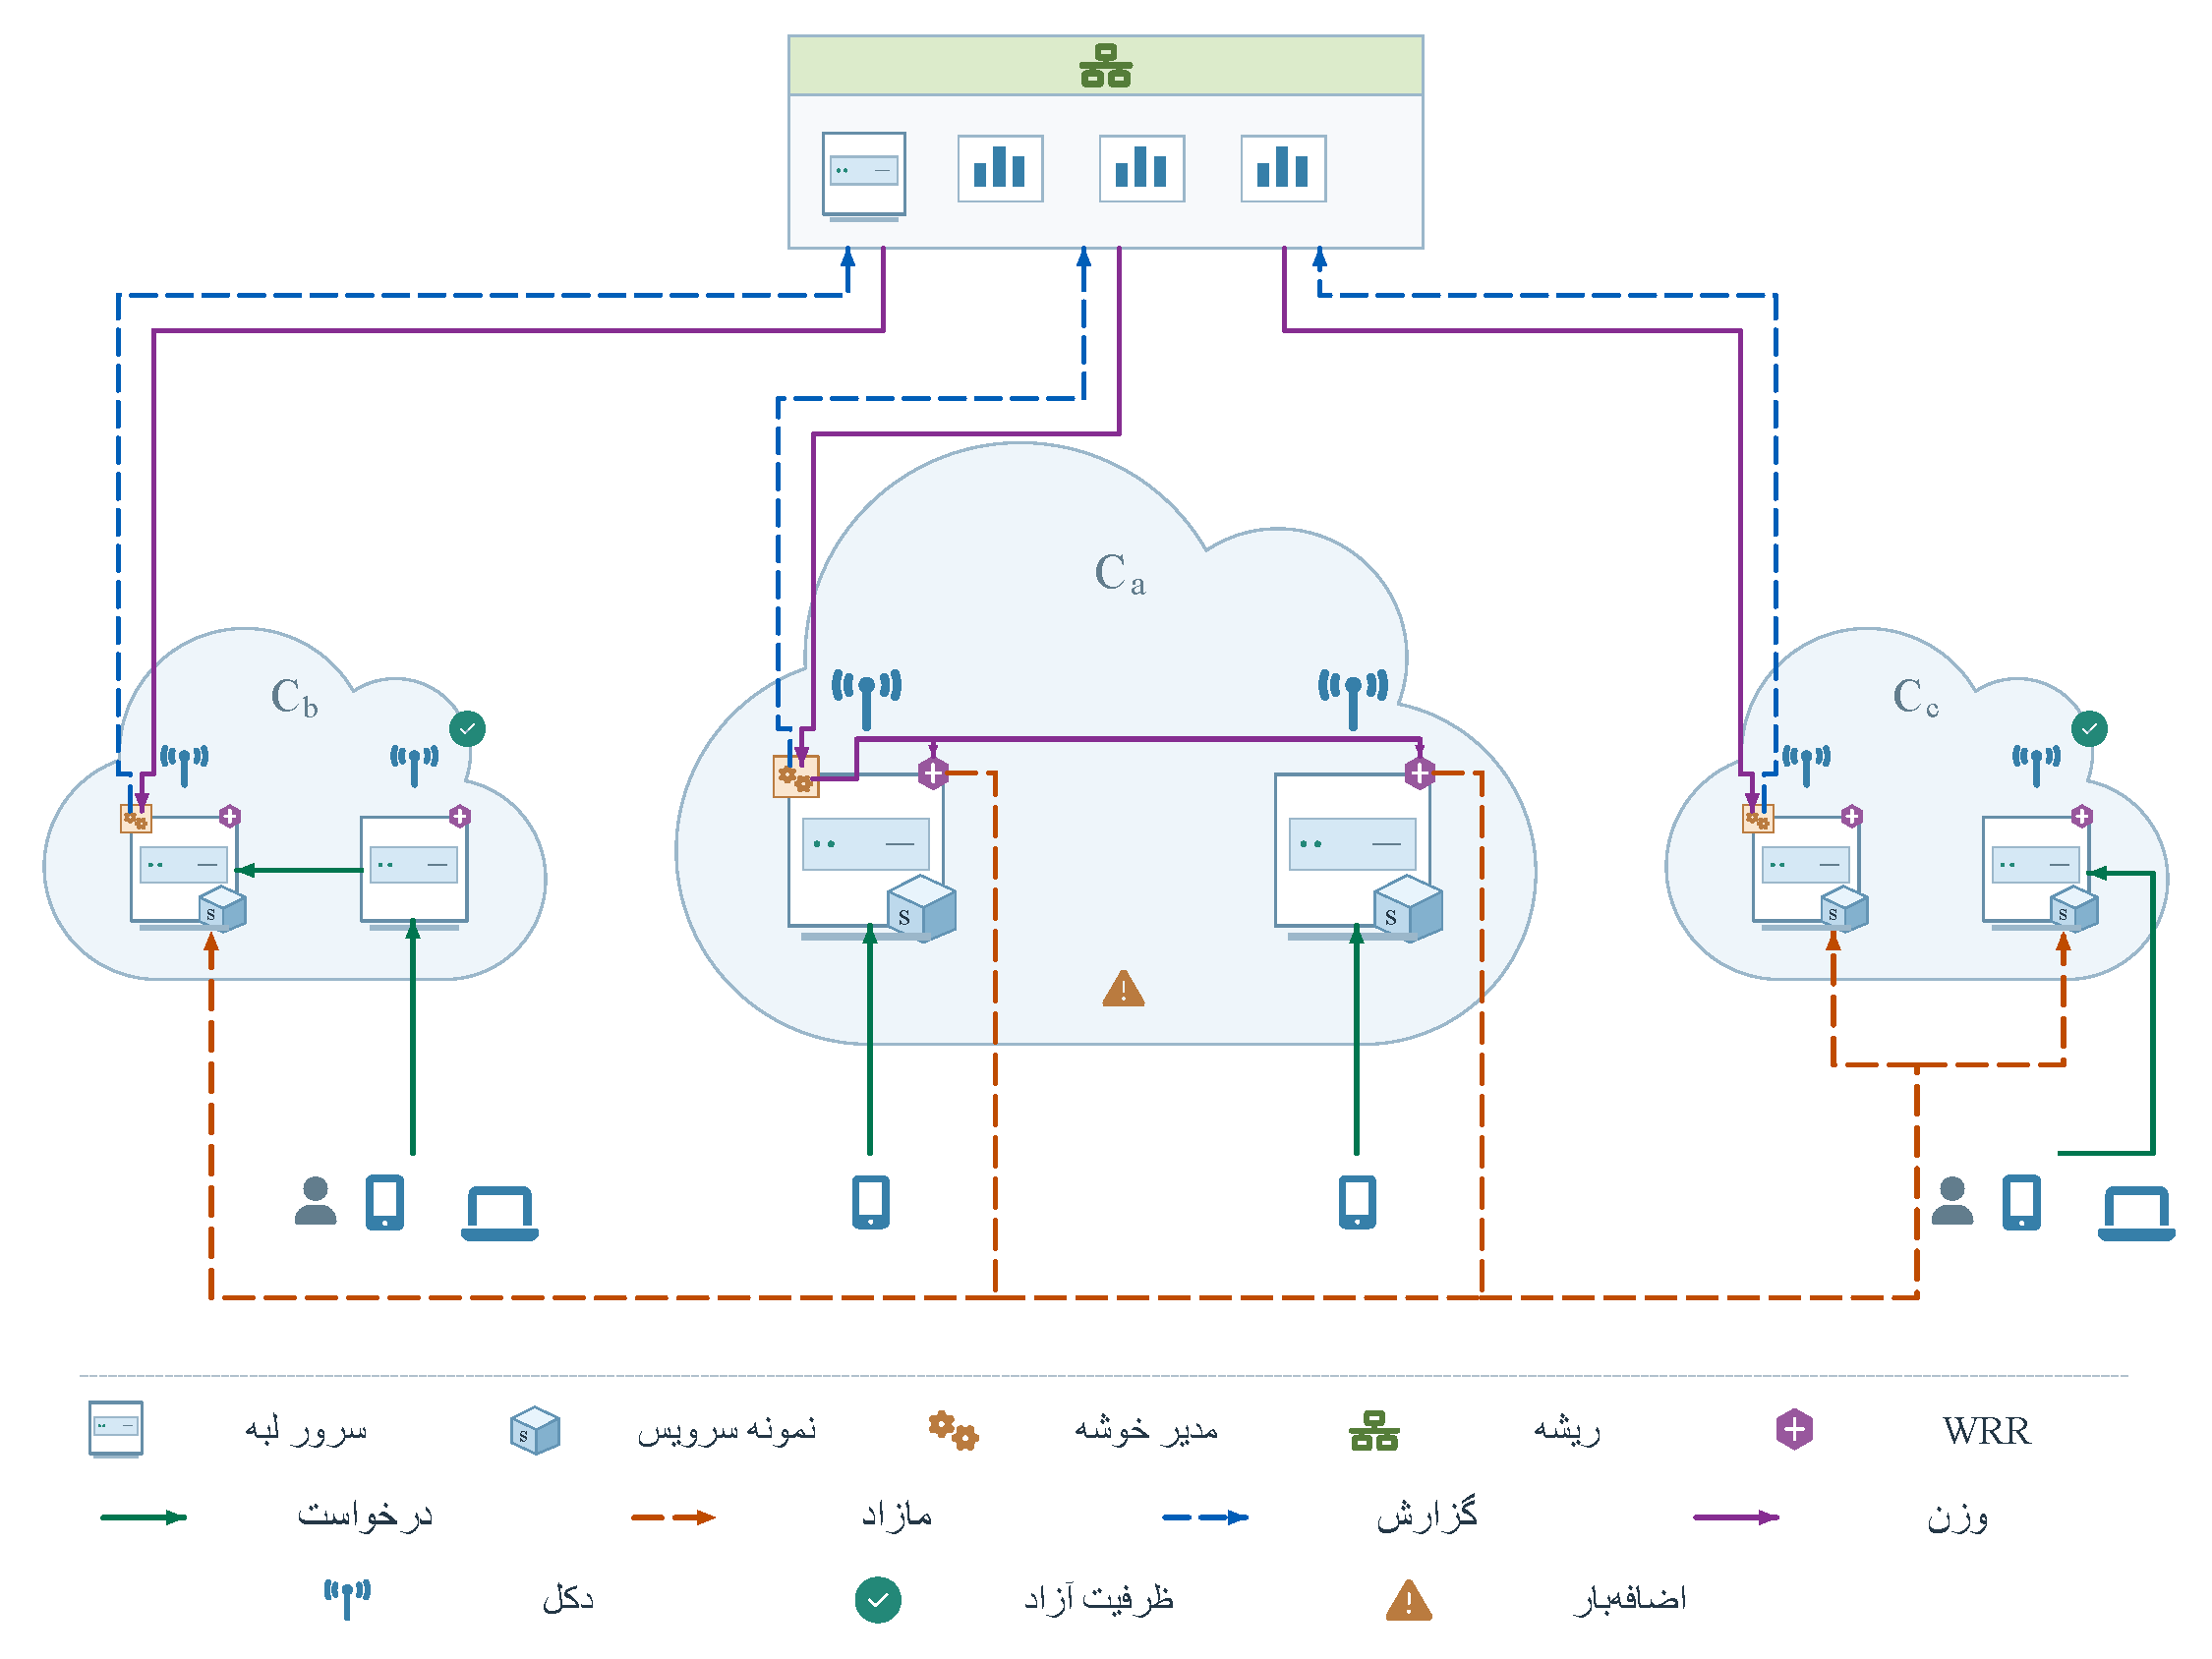
\includegraphics[width=\linewidth]{figures/visio/v10/03-campus-example.pdf}
\caption[مثال سه خوشه با یک لبه بدون سرویس]{سناریوی سه خوشه و شش سرور لبه. هر نماد بدنه، یک سرور است و مکعب، نمونه سرویس را نشان می‌دهد. لبه سمت راست خوشه $C_b$، یعنی $B_2$، مکعب سرویس ندارد و درخواست را به $B_1$ می‌فرستد. ورود کاربران به خوشه‌ها مستقل است. مسیر نارنجی پایین، مجموع ارسال مازاد مبدأهای $C_a$ به مقصدهای خارجی را نشان می‌دهد.}
\label{fig:campus-example}
\end{figure}

\subsubsection{ورودی‌ها و ترتیب محاسبه}

دو جدول زیر داده‌های مسئله را مشخص می‌کنند. پنجره پایش $\Delta=5$ ثانیه، حاشیه اطمینان $\varepsilon=0.1$، ضریب هزینه $\kappa_s=1$ و جریمه شکست $P_s=1$ ثانیه است. در این چرخه، نسبت شکست همه مسیرها و مازاد صف اندازه‌گیری‌شده صفرند؛ پس هزینه ثابت هر مسیر برابر میانگین پینگ همان مسیر است.

\Needspace{12\baselineskip}
\begin{longtable}{>{\centering\arraybackslash}p{1.8cm}>{\centering\arraybackslash}p{2.3cm}>{\centering\arraybackslash}p{1.9cm}>{\centering\arraybackslash}p{3.1cm}>{\centering\arraybackslash}p{3.6cm}}
\caption{استقرار سرویس و داده پردازنده در پنجره قبلی}\label{tab:example-input-hosts}\\
\toprule لبه & نمونه سرویس & هسته $g$ & پردازش پایان‌یافته $N^{\mathrm{proc}}$ & مصرف پردازنده $T^{\mathrm{CPU}}$ \\
\midrule\endfirsthead
\multicolumn{5}{c}{ادامه جدول \ref{tab:example-input-hosts}}\\
\toprule لبه & نمونه سرویس & هسته & پردازش پایان‌یافته & مصرف پردازنده \\
\midrule\endhead\bottomrule\endfoot
$A_1$ & دارد & $2$ & $450$ & $9$ \\
$A_2$ & دارد & $1$ & $270$ & $4.5$ \\
$B_1$ & دارد & $2$ & $285$ & $5.7$ \\
$B_2$ & ندارد & \lr{---} & \lr{---} & \lr{---} \\
$C_1$ & دارد & $2$ & $352$ & $7.04$ \\
$C_2$ & دارد & $1$ & $237$ & $3.95$ \\
\end{longtable}
مصرف پردازنده بر حسب هسته‌ثانیه است و همه ستون‌های پردازشی به کانتینر سرویس $s$ مربوط‌اند. خط تیره در سطر $B_2$ یعنی چنین کانتینری وجود ندارد؛ ظرفیت کل خود سرور صفر فرض نشده است. شمار پردازش‌های پایان‌یافته، همه مبدأهای محلی و خارجی را پوشش می‌دهد و به شمار ارسال یک مبدأ محدود نیست.

\Needspace{12\baselineskip}
\begin{longtable}{>{\centering\arraybackslash}p{1.8cm}>{\centering\arraybackslash}p{3.2cm}>{\centering\arraybackslash}p{3.7cm}>{\centering\arraybackslash}p{3.7cm}}
\caption{تقاضای مبدأها و میانگین پینگ به مقصدهای محلی}\label{tab:example-input-sources}\\
\toprule مبدأ & آغاز تلاش در پنجره $A^{\mathrm{src}}$ & پینگ به مقصد اول & پینگ به مقصد دوم \\
\midrule\endfirsthead
\multicolumn{4}{c}{ادامه جدول \ref{tab:example-input-sources}}\\
\toprule مبدأ & آغاز تلاش & پینگ مقصد اول & پینگ مقصد دوم \\
\midrule\endhead\bottomrule\endfoot
$A_1$ & $612$ & $1$ & $6$ \\
$A_2$ & $408$ & $6$ & $1$ \\
$B_1$ & $180$ & $1$ & \lr{---} \\
$B_2$ & $120$ & $6$ & \lr{---} \\
$C_1$ & $288$ & $1$ & $6$ \\
$C_2$ & $192$ & $6$ & $1$ \\
\end{longtable}
پینگ‌ها بر حسب میلی‌ثانیه‌اند و در هزینه به ثانیه تبدیل می‌شوند. مقصدهای محلی در $C_a$ برابر $(A_1,A_2)$، در $C_b$ فقط $B_1$ و در $C_c$ برابر $(C_1,C_2)$ هستند. برای هم‌میزبانی مبدأ و مقصد، مقدار $1$ میلی‌ثانیه نماینده مسیر محلی فراخوانی سرویس است. اتصال و مجوز دسترسی به همه مقصدهای نشان‌داده‌شده فراهم فرض می‌شود.

مدیر هر خوشه ابتدا سطر مبدأ شماره ۱ و سپس سطر شماره ۲ را حل می‌کند. نرخ‌های تقاضا از تقسیم شمار آغاز تلاش بر $5$ به دست می‌آیند:
\begin{equation}
 \boldsymbol D=(122.4,81.6,36,24,57.6,38.4),\qquad
 (D_{as},D_{bs},D_{cs})=(204,60,96).
\end{equation}
شمار آغاز تلاش و شمار پردازش پایان‌یافته دو شمارنده متفاوت‌اند. درخواست‌های در حال اجرا در مرز پنجره و جابه‌جایی میان خوشه‌ها سبب می‌شوند این دو شمار در یک سطر یا یک پنجره لزوما برابر نباشند.

\subsubsection{برآورد ظرفیت و تعیین سهم محلی}

برای نمونه $A_2$، روابط برآورد خطی چنین نتیجه می‌دهند:
\begin{equation}
 u_{sA_2}=\frac{4.5}{1\times5}=0.9,\qquad
 y_{sA_2}=\frac{270}{5}=54,\qquad
 \mu_{sA_2}=\frac{54}{0.9}=60.
\end{equation}
به همین ترتیب، با ترتیب مقصدهای $(A_1,A_2,B_1,C_1,C_2)$ داریم
\begin{align}
 \boldsymbol u&=(0.9,0.9,0.57,0.704,0.79),\\
 \boldsymbol\mu&=(100,60,100,100,60),\\
 \boldsymbol U&=(1-\varepsilon)\boldsymbol\mu=(90,54,90,90,54),\\
 (K_{as},K_{bs},K_{cs})&=(144,90,144).
\end{align}
واحد ظرفیت و نرخ، درخواست بر ثانیه است. چون $B_2$ نمونه سرویس ندارد، در جمع ظرفیت خوشه $C_b$ وارد نمی‌شود. با مقایسه تقاضا و ظرفیت محلی، نتیجه زیر به دست می‌آید:
\begin{align}
 (\eta_{as},\eta_{bs},\eta_{cs})&=(12/17,1,1),\\
 \boldsymbol\ell&=(86.4,57.6,36,24,57.6,38.4),\\
 \boldsymbol z&=(36,24,0,0,0,0).
\end{align}
پس فقط مبدأهای $C_a$ مازاد دارند و مجموع نرخ خارجی برابر $60$ است. خوشه‌های $C_b$ و $C_c$ ابتدا تقاضای مبدأهای خود را رزرو می‌کنند و سپس ظرفیت باقی‌مانده را به ریشه گزارش می‌دهند.

\subsubsection{حل مدیرهای خوشه}

در این مثال $\kappa_s=1$ است. برای کوتاه شدن نوشتن دستگاه‌ها، مشتق هزینه یک مقصد با ظرفیت $\mu$ و هزینه ثابت $d$ را چنین می‌نویسیم:
\begin{equation}
 G_{\mu,d}(r)=\frac{r(2\mu-r)}{(\mu-r)^2}+2dr.
\end{equation}
در جواب داخلی، مشتق مقصدها برابر $\nu$ و در مقصد روی سقف، $G_{\mu,d}(r)\leq\nu$ است. تخصیص سطرهای قبلی از سقف باقی‌مانده کم می‌شود، اما $\mu$ ثابت می‌ماند.

\paragraph{خوشه همراه اول.}
برای مبدأ $A_1$، سقف‌ها $(90,54)$ هستند و دستگاه به صورت زیر است:
\begin{equation}
\left\{\begin{aligned}
 \frac{r_1(200-r_1)}{(100-r_1)^2}+0.002r_1&=\nu,\\
 \frac{r_2(120-r_2)}{(60-r_2)^2}+0.012r_2&=\nu,\\
 r_1+r_2&=86.4.
\end{aligned}\right.
\end{equation}
با جایگذاری $r_2=86.4-r_1$ و حل در بازه مجاز، جواب و وزن شرطی محلی عبارت‌اند از
\begin{align}
 \boldsymbol r_{A_1}&\simeq(54.504863,31.895137),\qquad \nu\simeq3.940377,\\
 \boldsymbol w_{A_1}&=\boldsymbol r_{A_1}/86.4\simeq(0.630843,0.369157).
\end{align}
هر دو نرخ زیر سقف‌اند. برای مبدأ $A_2$، سقف باقی‌مانده $(35.495137,22.104863)$ است و مجموع آن دقیقا به نرخ محلی $57.6$ می‌رسد. بنابراین، جواب این سطر مستقیما از قید مجموع و سقف‌ها مشخص می‌شود:
\begin{align}
 \boldsymbol r_{A_2}&\simeq(35.495137,22.104863),\\
 \boldsymbol w_{A_2}&\simeq(0.616235,0.383765).
\end{align}
در این سطر، هزینه‌های ثابت به‌ترتیب $0.006$ و $0.001$ هستند. مشتق‌ها روی دو سقف تقریبا $1.829281$ و $1.551101$ می‌شوند؛ انتخاب $\nu=2$ هر دو نامساوی سقف را برقرار می‌کند. مجموع تخصیص محلی $C_a$ برابر $(90,54)$ است و ظرفیت عادی آزاد ندارد.

\paragraph{خوشه ایرانسل و لبه بدون سرویس.}
تنها مقصد محلی سرویس در این خوشه $B_1$ است. برای مبدأ $B_1$، قید مجموع نرخ را برابر $36$ و برای مبدأ $B_2$ آن را برابر $24$ قرار می‌دهد. نرخ دوم از سقف باقی‌مانده $90-36=54$ کمتر است؛ در نتیجه
\begin{equation}
 r_{B_1\rightarrow B_1}=36,\qquad
 r_{B_2\rightarrow B_1}=24,\qquad
 w_{B_1\rightarrow B_1}=w_{B_2\rightarrow B_1}=1.
\end{equation}
برای این دو سطر، مقدارهای $\nu$ به‌ترتیب $G_{100,0.001}(36)=1.513406$ و $G_{100,0.006}(24)\simeq1.019302$ هستند. هر دو جواب داخلی و مجازند. لبه $B_2$ فقط وزن ارسال را به کار می‌برد؛ مجموع نرخ پردازش محلی روی کانتینر $B_1$ برابر $60$ است.

\paragraph{خوشه رایتل.}
برای مبدأ $C_1$، دستگاه با سقف $(90,54)$ عبارت است از
\begin{equation}
 G_{100,0.001}(r_1)=G_{60,0.006}(r_2)=\nu,\qquad r_1+r_2=57.6.
\end{equation}
حل آن، $\boldsymbol r_{C_1}\simeq(36.871360,20.728640)$ و $\nu\simeq1.583011$ است. پس سقف سطر بعد $(53.128640,33.271360)$ می‌شود. برای مبدأ $C_2$ داریم
\begin{equation}
 G_{100,0.006}(r_1)=G_{60,0.001}(r_2)=\nu,\qquad r_1+r_2=38.4.
\end{equation}
جواب این سطر $\boldsymbol r_{C_2}\simeq(22.132591,16.267409)$ و $\nu\simeq0.914849$ است. هر دو سطر زیر سقف‌های مربوط به خود قرار دارند. وزن‌ها و مجموع تخصیص محلی این خوشه عبارت‌اند از
\begin{align}
 \boldsymbol w_{C_1}&\simeq(0.640128,0.359872),\\
 \boldsymbol w_{C_2}&\simeq(0.576370,0.423630),\\
 \boldsymbol R^{\mathrm{plan}}_c&\simeq(59.003950,36.996050).
\end{align}

\subsubsection{حل ریشه و ترکیب وزن‌ها}

هر مدیر، ظرفیت خالی همان کانتینرها را پس از رزرو محلی محاسبه می‌کند. با ترتیب پنج مقصد اعلام‌شده داریم
\begin{equation}
 \boldsymbol S=\boldsymbol U-\boldsymbol R^{\mathrm{plan}}
 \simeq(0,0,30,30.996050,17.003950).
\end{equation}
در نتیجه $A_{as}=0$، $A_{bs}=30$ و $A_{cs}=48$ است. مجموعه پذیرنده‌ها $\mathcal R_s=\{b,c\}$، مجموع ظرفیت آزاد $V_s=78$ و نرخ مازاد $O_s=60$ می‌شود. چون $O_s<V_s$، ریشه از شاخه عادی استفاده می‌کند:
\begin{equation}
 (\pi_{sa},\pi_{sb},\pi_{sc})=(0,5/13,8/13).
\end{equation}
خوشه $C_b$ یک نمونه دارد، پس $v_{sb1}=1$ است. سهم دو نمونه خوشه $C_c$ از تقسیم ظرفیت خالی هر کدام بر $48$ به دست می‌آید:
\begin{equation}
 (v_{sc1},v_{sc2})\simeq(0.645751,0.354249).
\end{equation}
نرخ کل خارجی به $C_b$ برابر $60(5/13)=23.076923$ و به $C_c$ برابر $60(8/13)=36.923077$ است. ریشه همین سهم‌ها را به مدیر مبدأ می‌دهد.

مدیر $C_a$، وزن محلی هر مبدأ را در $12/17$ و سهم خارجی آن را در $5/17$ ضرب می‌کند. برای نمونه، دو درایه خروجی مبدأ $A_1$ چنین محاسبه می‌شوند:
\begin{align}
 W_{A_1,s,a,1}&\simeq(12/17)(0.630843)=0.445301,\\
 W_{A_1,s,b,1}&=(5/17)(5/13)(1)\simeq0.113122.
\end{align}
برای هر مقصد خارجی، حاصل‌ضرب سهم خوشه و نمونه برابر $S_i/78$ است. بنابراین وزن خارجی هر مبدأ $C_a$ برابر $(5/17)S_i/78$ می‌شود. مبدأهای $C_b$ و $C_c$ مازاد ندارند و وزن‌هایشان فقط از حل محلی می‌آید.

\paragraph{کنترل مجموع و ظرفیت.}
وزن‌های هر سطر نامنفی‌اند و مجموع آن‌ها یک است. برای سطرهای $C_a$، مجموع وزن محلی $12/17$ و مجموع وزن خارجی $5/17$ است. نرخ مقصد از جمع سهم همه مبدأها به دست می‌آید، نه فقط از یک مبدأ:
\begin{equation}
 L_i=\sum_e D_{es}W_{esi}.
\end{equation}
با ترتیب $(A_1,A_2,B_1,C_1,C_2)$، نرخ‌های کل حاصل عبارت‌اند از
\begin{equation}
 \boldsymbol L\simeq(90,54,83.076923,82.847065,50.076011)
 \ \leq\ (90,54,90,90,54).
\end{equation}
مجموع نرخ‌ها $360$ و برابر مجموع تقاضای شش مبدأ است. نرخ خارجی هر مقصد $(60/78)S_i$ است و از ظرفیت آزاد آن کمتر می‌ماند. این بررسی برای داده ثابت همین چرخه است.

\subsubsection{حالت‌های دیگر همین استقرار}

در حالت‌های زیر، استقرار پنج نمونه ثابت می‌ماند و فقط ورودی چرخه تغییر می‌کند. سقف خوشه‌ها همچنان $(144,90,144)$ است، مگر آنکه خرابی مقصد ذکر شود.
\begin{enumerate}[label=\arabic*.,leftmargin=*]
\item \textbf{ظرفیت محلی کافی یا برابری با سقف.}
با تقاضای $(100,60,96)$، همه درخواست‌ها محلی‌اند و وزن‌های دو مبدأ $C_a$ به‌ترتیب $(0.639152,0.360848)$ و $(0.578102,0.421898)$ می‌شوند. با تقاضای $C_a$ برابر $144$ نیز سهم محلی یک است و مسیر خارجی فعال نمی‌شود.
\item \textbf{کمبود ظرفیت کل.}
با تقاضای $(330,75,120)$، مازاد $C_a$ برابر $186$ و ظرفیت آزاد پذیرنده‌ها $(15,24)$ است. اضافه بر ظرفیت، یعنی $147$، به دو سهم $73.5$ تقسیم می‌شود؛ در نتیجه نرخ خارجی $C_b$ برابر $88.5$ و نرخ خارجی $C_c$ برابر $97.5$ است. نرخ نهایی تنها میزبان $C_b$ به $163.5$ و دو میزبان $C_c$ به $(126.75,90.75)$ می‌رسد. این توزیع موقت، ظرفیت پردازشی تازه ایجاد نمی‌کند و به افزایش ظرفیت نیاز دارد.
\item \textbf{نبود پذیرنده خارجی.}
با تقاضای $(200,100,170)$، هر سه خوشه مازاد دارند. مازاد $C_a$ برابر $56$ است و موقتا به دو سهم $28$ میان میزبان‌های همان سرویس تقسیم می‌شود؛ بار آن‌ها $(118,82)$ خواهد شد. لبه بدون سرویس $B_2$ حتی در این شاخه مقصد پردازش نیست.
\item \textbf{خرابی یا نبود تقاضا.}
با خرابی $A_2$ و تقاضای $(100,60,96)$، ظرفیت $C_a$ به $90$ می‌رسد؛ وزن مقصد خراب صفر و نرخ خارجی $10$ می‌شود. اگر تقاضای $C_a$ صفر باشد، مبدأهای آن ارسالی ندارند و وزنی از تقسیم بر نرخ صفر ساخته نمی‌شود.
\item \textbf{افزایش خطای مسیر.}
در حالت تقاضای محلی $C_a$ برابر $100$، افزایش نسبت شکست مسیر $A_1$ به $A_1$ از صفر به $0.1$، هزینه ثابت آن را از $0.001$ به $0.101$ ثانیه می‌رساند. با ثابت ماندن سایر ورودی‌های همان سطر، وزن این مقصد از $0.639152$ به $0.402205$ کاهش می‌یابد.
\end{enumerate}

\Needspace{20\baselineskip}
\subsubsection{ماتریس نهایی وزن‌ها}

ماتریس زیر خروجی داده‌های دو جدول ورودی است. هر سطر یک مبدأ و هر ستون یک مقصد دارای سرویس را نشان می‌دهد. نرخ ارسال به هر مقصد، حاصل‌ضرب وزن در تقاضای همان سطر است.

\begin{equation}
\mathbf W_s\simeq
\bordermatrix{
 & A_1 & A_2 & B_1 & C_1 & C_2\cr
A_1 & 0.445301 & 0.260581 & 0.113122 & 0.116878 & 0.064117\cr
A_2 & 0.434989 & 0.270893 & 0.113122 & 0.116878 & 0.064117\cr
B_1 & 0 & 0 & 1 & 0 & 0\cr
B_2 & 0 & 0 & 1 & 0 & 0\cr
C_1 & 0 & 0 & 0 & 0.640128 & 0.359872\cr
C_2 & 0 & 0 & 0 & 0.576370 & 0.423630\cr
}.
\label{eq:example-weight-matrix}
\end{equation}
لبه $B_2$ فرستنده است و سطر دارد، اما چون سرویس ندارد، ستون ندارد. دو سطر خوشه $C_b$ به علت وجود تنها یک مقصد محلی برابرند؛ وزن‌های مبدأهای دیگر متفاوت‌اند. کنترل مجموع سطرها و ظرفیت با مقادیر کامل پیش از گرد کردن انجام شده است.

مدیر خوشه، سطر هر مبدأ را به همان لبه می‌رساند تا با \lr{WRR} اجرا شود.


\section{جمع‌بندی فصل}

مدیر خوشه، ظرفیت نمونه‌ها را برآورد و بار محلی را با روش هزینه پایه تخصیص می‌دهد. ریشه سهم مقصدهای خارجی را از ظرفیت آزاد پس از رزرو محلی می‌سازد. تا وقتی ظرفیت داخلی کافی است، وزن خارجی صفر می‌ماند؛ در غیر این صورت، فقط مازاد از سهم ریشه پیروی می‌کند. مدیر مبدأ جدول نهایی را رویدادی منتشر می‌کند و لبه آن را با نوبت‌گردشی وزن‌دار اجرا می‌کند.
